% \iffalse
%
% Copyright 2016-2017, Association for Computing Machinery
% This work may be distributed and/or modified under the
% conditions of the LaTeX Project Public License, either
% version 1.3 of this license or (at your option) any
% later version.
% The latest version of the license is in
%    http://www.latex-project.org/lppl.txt
% and version 1.3 or later is part of all distributions of
% LaTeX version 2005/12/01 or later.
%
% This work has the LPPL maintenance status `maintained'.
%
% The Current Maintainer of this work is Boris Veytsman,
% <borisv@lk.net>
%
% This work consists of the file acmart.dtx and the
% derived file acmart.cls, and
%
% \fi
%
%
%% \CharacterTable
%%  {Upper-case    \A\B\C\D\E\F\G\H\I\J\K\L\M\N\O\P\Q\R\S\T\U\V\W\X\Y\Z
%%   Lower-case    \a\b\c\d\e\f\g\h\i\j\k\l\m\n\o\p\q\r\s\t\u\v\w\x\y\z
%%   Digits        \0\1\2\3\4\5\6\7\8\9
%%   Exclamation   \!     Double quote  \"     Hash (number) \#
%%   Dollar        \$     Percent       \%     Ampersand     \&
%%   Acute accent  \'     Left paren    \(     Right paren   \)
%%   Asterisk      \*     Plus          \+     Comma         \,
%%   Minus         \-     Point         \.     Solidus       \/
%%   Colon         \:     Semicolon     \;     Less than     \<
%%   Equals        \=     Greater than  \>     Question mark \?
%%   Commercial at \@     Left bracket  \[     Backslash     \\
%%   Right bracket \]     Circumflex    \^     Underscore    \_
%%   Grave accent  \`     Left brace    \{     Vertical bar  \|
%%   Right brace   \}     Tilde         \~}
%
%
% \MakeShortVerb{|}
% \GetFileInfo{acmart.dtx}
% \newcommand{\progname}[1]{\textsf{#1}}
% \title{\LaTeX{} Class for \emph{Association for Computing
% Machinery}\thanks{\copyright 2016--2017, Association for Computing Machinery}}
% \author{Boris Veytsman\thanks{%
% \href{mailto:borisv@lk.net}{\texttt{borisv@lk.net}},
% \href{mailto:boris@varphi.com}{\texttt{boris@varphi.com}}}}
% \date{\filedate, \fileversion}
% \maketitle
% \begin{abstract}
%   This package provides a class for typesetting publications of
%   Association for Computing Machinery.
% \end{abstract}
% \tableofcontents
%
% \clearpage
%
%\section{Introduction}
%\label{sec:intro}
%
% Association for Computing Machinery is the world's largest
% educational and scientific computing society, which delivers
% resources that advance computing as a science and a
% profession\footnote{\url{http://www.acm.org/}}.  It was one of the
% earily adopters of \TeX\ for its typesetting.
%
% It provided several different classes for a number of journal and
% conference proceedings.  Unfortunately during the years since these
% classes were written, the code was patched many times, and the
% support of the different versions of the classes became difficult.
%
% This package provides the uniform interface for all ACM
% publications.  It is intended to replace all different classes and
% packages and provide an up to date \LaTeX\ package.
%
% The package uses only free \TeX\ packages and fonts included in \TeX
% Live, Mik\TeX\ and other popular \TeX\ distributions.  It is
% intended to be published in these distributions itself, which
% minimizes users' efforts in the installation and support of the
% package.
%
%  I am grateful to
%  Matthew Fluet, 
%  John Owens,
%  Craig Rodkin,
%  Bernard Rous,
%  David Shamma,
%  Stephen Spencer
%  and many others for their invaluable help.
%
% The development version of the package is available at
% \url{https://github.com/borisveytsman/acmart}. 
%
%\section{User's guide}
%\label{sec:ug}
%
%
%\subsection{Installation}
%\label{sec:ug_install}
%
% Most probably, you already have this package installed in your
% favorite \TeX\ distribution;  if not, you may want to upgrade.  You
% may need to upgrade it anyway since the package uses a number
% relatively recent packages, especially the ones related to the
% fonts.
%
% If you decide to install the package yourself, follow the standard
% rules:
% \begin{enumerate}
% \item Run \progname{latex} on |acmart.ins|.  This will produce the file
% |acmart.cls|.
% \item Put the file |acmart.cls| and the bibligoraphy files |*.bst|
%   to the places where \LaTeX{} can find them (see \cite{TeXFAQ} or
%   the documentation for your \TeX{} system).\label{item:install}
% \item Update the database of file names.  Again, see \cite{TeXFAQ}
% or the documentation for your \TeX{} system for the system-specific
% details.\label{item:update}
% \item The file |acmart.pdf| provides the documentation for the
% package (this is the file you are probably reading now).
% \end{enumerate}
% As an alternative to items~\ref{item:install} and~\ref{item:update}
% you can just put the files in the working directory where your
% |.tex| file is.
%
%
% The class uses a number of other packages.  They are included in all
% major \TeX\ distributions (\TeX Live, Mac\TeX, Mik\TeX) of 2015 and
% later, so you probably have them installed.  Just in case here is
% the list of these packages:
% \begin{itemize}
% \item \textsl{amscls}, \url{http://www.ctan.org/pkg/amscls}
% \item \textsl{amsfonts}, \url{http://www.ctan.org/pkg/amsfonts}
% \item \textsl{amsmath}, \url{http://www.ctan.org/pkg/amsmath}
% \item \textsl{binhex}, \url{http://www.ctan.org/pkg/binhex}
% \item \textsl{caption}, \url{http://www.ctan.org/pkg/caption}
% \item \textsl{comment}, \url{http://www.ctan.org/pkg/comment}
% \item \textsl{environ}, \url{http://www.ctan.org/pkg/environ}
% \item \textsl{fancyhdr}, \url{http://www.ctan.org/pkg/fancyhdr}
% \item \textsl{float}, \url{http://www.ctan.org/pkg/float}
% \item \textsl{fontaxes}, \url{http://www.ctan.org/pkg/fontaxes}
% \item \textsl{geometry}, \url{http://www.ctan.org/pkg/geometry}
% \item \textsl{graphics}, \url{http://www.ctan.org/pkg/graphics}
% \item \textsl{hyperref}, \url{http://www.ctan.org/pkg/hyperref}
% \item \textsl{ifluatex}, \url{http://www.ctan.org/pkg/ifluatex}
% \item \textsl{ifxetex}, \url{http://www.ctan.org/pkg/ifxetex}
% \item \textsl{inconsolata}, \url{http://www.ctan.org/pkg/inconsolata}
% \item \textsl{latex-tools}, \url{http://www.ctan.org/pkg/latex-tools}
% \item \textsl{libertine}, \url{http://www.ctan.org/pkg/libertine}
% \item \textsl{manyfoot}, \url{http://www.ctan.org/pkg/manyfoot}
% \item \textsl{microtype}, \url{http://www.ctan.org/pkg/microtype}
% \item \textsl{ms}, \url{http://www.ctan.org/pkg/ms}
% \item \textsl{mweights}, \url{http://www.ctan.org/pkg/mweights}
% \item \textsl{natbib}, \url{http://www.ctan.org/pkg/natbib}
% \item \textsl{nccfoots}, \url{http://www.ctan.org/pkg/nccfoots}
% \item \textsl{newtx}, \url{http://www.ctan.org/pkg/newtx}
% \item \textsl{oberdiek}, \url{http://www.ctan.org/pkg/oberdiek}
% \item \textsl{pdftex-def}, \url{http://www.ctan.org/pkg/pdftex-def}
% \item \textsl{setspace}, \url{http://www.ctan.org/pkg/setspace}
% \item \textsl{totpages}, \url{http://www.ctan.org/pkg/totpages}
% \item \textsl{trimspaces}, \url{http://www.ctan.org/pkg/trimspaces}
% \item \textsl{upquote}, \url{http://www.ctan.org/pkg/upquote}
% \item \textsl{url}, \url{http://www.ctan.org/pkg/url}
% \item \textsl{xcolor}, \url{http://www.ctan.org/pkg/xcolor}
% \item \textsl{xkeyval}, \url{http://www.ctan.org/pkg/xkeyval}
% \end{itemize}
% 
%
%\subsection{Invocation and options}
%\label{sec:invocation}
%
% To use the class put in the premable of your document
% \begin{quote}
%   \cs{documentclass}\oarg{options}|{acmart}|
% \end{quote}
% There are several options corresponding to the type of the document and
% its general appearance.  They are described below.  Generally
% speaking, the options have |key=value| forms, for example
% \begin{verbatim}
% \documentclass[format=acmsmall, screen=true, review=false]{acmart}
% \end{verbatim}
%
%
% The option |format| describes the format of the output.  There are
% several possible values for this option, for example,
% \begin{verbatim}
%   \documentclass[format=acmtog]{acmart}
% \end{verbatim}
% Actually the words |format=| can be omitted, e.g.,
% \begin{verbatim}
%   \documentclass[acmtog, review=false]{acmart}
% \end{verbatim}
% The possible formats are listed in
% Table~\ref{tab:opts_format}.  Note that formats starting with |acm|
% are intended for journals and transactions, while formats starting
% with |sig| are intended for proceedings published as books.
%
% \begin{table}
%   \centering
%   \caption{The possible values for the \texttt{format} option}
%   \label{tab:opts_format}
%   \begin{tabularx}{\textwidth}{>{\ttfamily}lX}
%     \toprule
%     \normalfont Value & Meaning\\
%     \midrule
%     manuscript  & A manuscript. This is the default \\
%   acmsmall & Small single column format, used for CIE, CSUR, JACM, JDIQ, JEA, JERIC,
%            JETC, TAAS, TACCESS, TACO, TALG, TALLIP (formerly TALIP), TCPS,
%            TEAC, TECS, TIIS, TISSEC, TIST, TKDD, TMIS, TOCE, TOCHI, TOCL,
%            TOCS, TOCT, TODAES, TODS, TOIS, TOIT, TOMACS, TOMM (formerly
%            TOMCCAP), TOMPECS, TOMS, TOPC, TOPLAS, TOPS,
%            TOS, TOSEM, TOSN, TRETS,
%            TSAS, TSC, TSLP, TWEB\@. \\
%           acmlarge  & Large single column format, used for
%           IMWUT, JOCCH, PACMPL, TAP \\
%            acmtog   & Large double column format, used for
%          TOG\\
%           sigconf & Proceedings format for most of ACM
%          conferences (with the exceptions listed below)\\
%           siggraph & Proceedings format for SIGGRAPH and SIGGRAPH
%          Asia conferences, published in ACM Transactions on Graphics
%          journal issues \\
%            sigplan & Proceedings format for SIGPLAN conferences\\
%            sigchi  & Proceedings format for SIGCHI conferences\\
%           sigchi-a & Format for SIGCHI extended abstract\\
%   \bottomrule
%   \end{tabularx}
% \end{table}
%
% There are several Boolean options which can take |true| or |false|
% values.  They are listed in Table~\ref{tab:opts_bool}.  The words
% |=true| can be omitted when setting the Boolean option, so instead of
% |screen=true| one can write just |screen|, for example,
% \begin{verbatim}
% \documentclass[acmsmall, screen, review]{acmart}
% \end{verbatim}
% The option
% |review| is useful when combined with the |manuscript| format
% option: it provides a version suitable for reviewers and
% copyeditors.  
%
% The option |screen| may in the future involve
% additional features  suitable for on-screen versions of the
% articles.  
% 
% The option |natbib| is used when the corresponding
% \BibTeX\ style is based on |natbib|.  In most cases you do not need
% to set it.  See
% Section~\ref{sec:ug_bibliography}.  
%
% The option |anonymous| is used
% for anonymous review process: all author information becomes
% obscured.  
%
% \begin{table}
%   \centering
%   \caption{Boolean options}
%   \label{tab:opts_bool}
%   \begin{tabularx}{\textwidth}{>{\ttfamily}l>{\ttfamily}lX}
%     \toprule
%     \normalfont Option & \normalfont Default & Meaning\\
%     \midrule
%     review & false & A review version: lines are numbered,
%     hyperlinks are colored\\
%     screen & false & A screen version: hyperlinks are colored\\
%     natbib & true & Whether to use |natbib| package (see
%     Section~\ref{sec:ug_bibliography})\\
%     anonymous & false & Whether to make author(s) anonymous\\
%     authorversion & false & Whether to generate a special
%     version for authors' personal use or posting (see
%     Section~\ref{sec:ug_topmatter})\\ 
%     \bottomrule
%   \end{tabularx}
% \end{table}
%
%
%
%\subsection{Topmatter commands}
%\label{sec:ug_topmatter}
%
% A number of commands set up \emph{top matter} information, or, in
% the computer science jargon, \emph{metadata} for the article.  They
% establish the publication name, article title, authors, doi and
% other data.  Some of these commands, like \cs{title} or \cs{author},
% should be put by the authors.  Others, like \cs{acmVolume} or
% \cs{acmDOI}---by the editors.  Below we describe these commands and
% mention who should issue them.  These macros should be used
% \emph{before} the \cs{maketitle} command.  Note that in the previous
% versions of ACM classes some of these commands should be used before
% \cs{maketitle}, and some after it. Now they all must be used before
% \cs{maketitle}.
%
%
% The class internally loads |amsart| class, so many top matter
% commands are inherited from |amsart|~\cite{Downes04:amsart}.
%
% \DescribeMacro{\acmJournal}%
% The macro \cs{acmJournal}\marg{shortName} sets the name of the
% journal or transaction for journals and transactions.  The argument
% is the short name of the publication \emph{in uppercase}, for
% example,
% \begin{verbatim}
% \acmJournal{TOMS}
% \end{verbatim}
% The currently recognized journals are listed in
% Table~\ref{tab:pubs}.  Note that conference proceedings published in
% \emph{book} form do not set this macro.
%
% \begin{table}
%   \centering
%   \caption{ACM publications and arguments of the \cs{acmJournal}
%   command}\footnotesize
%   \label{tab:pubs}
%   \begin{tabularx}{\textwidth}{>{\ttfamily}lX}
%     \toprule
%     \normalfont Abbreviation & Publication \\
%     \midrule
%     CIE & ACM Computers in Entertainment \\
%     CSUR & ACM Computing Surveys\\
%     IMWUT & PACM on Interactive, Mobile, Wearable and Ubiquitous
%     Technologies\\ 
%     JACM &  Journal of the ACM \\
%     JDIQ & ACM Journal of Data and Information Quality \\
%     JEA & ACM Journal of Experimental Algorithmics \\
%     JERIC & ACM Journal of Educational Resources in Computing\\
%     JETC & ACM Journal on Emerging Technologies in Computing Systems \\
%     JOCCH & ACM Journal on Computing and Cultural Heritage \\
%     PACMPL & PACM on Programming Languages \\
%     TAAS & ACM Transactions on Autonomous and Adaptive Systems\\
%     TACCESS & ACM Transactions on Accessible Computing\\
%     TACO & ACM Transactions on Architecture and Code Optimization \\
%     TALG & ACM Transactions on Algorithms \\
%     TALLIP & ACM Transactions on Asian and Low-Resource Language
%     Information Processing\\
%     TAP & ACM Transactions on Applied Perception \\
%     TCPS & ACM Transactions on Cyber-Physical Systems\\
%     TEAC & ACM Transactions on Economics and Computation\\
%     TECS & ACM Transactions on Embedded Computing Systems \\
%     TIIS & ACM Transactions on Interactive Intelligent Systems\\
%     TISSEC & ACM Transactions on Information and System Security\\
%     TIST & ACM Transactions on Intelligent Systems and Technology \\
%     TKDD & ACM Transactions on Knowledge Discovery from Data\\
%     TMIS & ACM Transactions on Management Information Systems\\
%     TOCE & ACM Transactions on Computing Education\\
%     TOCHI & ACM Transactions on Computer-Human Interaction\\
%     TOCL & ACM Transactions on Computational Logic\\
%     TOCS & ACM Transactions on Computer Systems  \\
%     TOCT & ACM Transactions on Computation Theory  \\
%     TODAES & ACM Transactions on Design Automation of Electronic Systems\\
%     TODS & ACM Transactions on Database Systems\\
%     TOG & ACM Transactions on Graphics\\
%     TOIS & ACM Transactions on Information Systems\\
%     TOIT & ACM Transactions on Internet Technology\\
%     TOMACS & ACM Transactions on Modeling and Computer Simulation \\
%     TOMM  & ACM Transactions on Multimedia Computing, Communications
%     and Applications \\
%     TOMPECS & ACM Transactions on Modeling and Performance Evaluation
%     of Computing Systems\\
%     TOMS & ACM Transactions on Mathematical Software\\
%     TOPC & ACM Transactions on Parallel Computing\\
%     TOPLAS & ACM Transactions on Programming Languages and Systems\\
%     TOPS & ACM Transactions on Privacy and Security\\
%     TOS & ACM Transactions on Storage\\
%     TOSEM & ACM Transactions on Software Engineering and Methodology\\
%     TOSN & ACM Transactions on Sensor Networks\\
%     TRETS & ACM Transactions on Reconfigurable Technology and Systems\\
%     TSAS & ACM Transactions on Spatial Algorithms and Systems\\
%     TSC & ACM Transactions on Social Computing\\
%     TSLP & ACM Transactions on Speech and Language Processing \\
%     TWEB & ACM Transactions on the Web\\
%   \bottomrule
%   \end{tabularx}
% \end{table}
%
% It is expected that this command is inserted by the author of the
% manuscript when she decides to which journal to submit the
% manuscript.
%
% \DescribeMacro{\acmConference}%
% The macro
% \cs{acmConference}\oarg{short name}\marg{name}\marg{date}\marg{venue} is
% used for conference proceedings published in the book form.  The
% arguments are the following:
% \begin{description}
% \item[short name:] the abbreviated name of the conference (optional).
% \item[name:] the name of the conference \emph{or} the name of the
% book as set by the editor.
% \item[date:] the date(s) of the conference.
% \item[venue:] the place of the conference.
% \end{description}
% Examples:
% \begin{verbatim}
% \acmConference[TD'15]{Technical Data Conference}{November
% 12--16}{Dallas, TX, USA}
% \acmConference{SA'15 Art Papers}{November 02--06, 2015}{Kobe, Japan}
% \end{verbatim}
%
%
% Normally this command is entered either by the editor or by the typesetter.
%
% \DescribeMacro{\title}
% The command |\title|, as in \progname{amsart} class, has two arguments:  one
% optional, and one mandatory:
% \begin{flushleft}
%   |\title[|\meta{ShortTitle}|]{|\meta{FullTitle}|}|
% \end{flushleft}
% The mandatory argument is the full title of the article.  The
% optional argument, if present, defines the shorter version of the
% title for running heads.  If the optional argument is absent, the
% full title is used instead.
%
% It is expected that this command is inserted by the author of the
% manuscript.
%
% \DescribeMacro{\subtitle}%
% Besides title, ACM classes allow subtitle, set with the
% \cs{subtitle}\marg{subtitle} macro.
%
% The commands for specification of authors are highly structured.
% The reason is, they serve double duty:  the authors' information is
% typeset in the manuscript, \emph{and} is used by the metadata
% extraction tools for indexing and cataloguing.  Therefore it is very
% important to follow the guidelines exactly.
%
% \DescribeMacro{\author}%
% \DescribeMacro{\orcid}
% \DescribeMacro{\affiliation}%
% \DescribeMacro{\email}%
% The basic commands are \cs{author}, \cs{orcid} (for the researchers
% registered with ORCID, \url{http://www.orcid.org/}), \cs{affiliation} and
% \cs{email}.  In the simplest case you enter them in this order:
% \begin{verbatim}
% \author{...}
% \orcid{...}
% \affiliation{...}
% \email{...}
% \end{verbatim}
% Do \emph{not} use \LaTeX\ \cs{and} macro! Each author deserves
% his or her own \cs{author} command.
%
% Note that some formats do not typset e-mails of ORCID identifiers.
% Do not worry: metadata tools will get them.  
%
% Sometimes an author has several affiliations.  In this case the
% \cs{affiliation} command should be repeated:
% \begin{verbatim}
% \author{...}
% \orcid{...}
% \affiliation{...}
% \affiliation{...}
% \email{...} 
% \end{verbatim}
% Similarly you can repeat \cs{email} command.
%
% You may have several authors with the same afifliation, different
% affiliations or overlapping affiliations (author~$A_1$ is affiliated
% with institutions $I_1$ and $I_2$, while author $A_2$ is affiliated
% with $I_2$ only, and author $A_3$ is affiliated with
% $I_1$ and $I_3$, \ldots).  The recommended solution is to put the
% \cs{affiliation} commands after each author, possibly repeating them:
% \begin{verbatim}
% \author{...}
% \orcid{...}
% \affiliation{...}
% \affiliation{...}
% \email{...} 
% \author{...}
% \orcid{...}
% \affiliation{...}
% \email{...}  
% \author{...}
% \orcid{...}
% \affiliation{...}
% \affiliation{...}
% \email{...} 
% \end{verbatim}
%  In some cases when several authors share the same affiliation you may
%  try to save the space using the format
% \begin{verbatim}
% \author{...}
% \email{...}
% \author{...}
% \email{...}
% \affiliation{...}
% \end{verbatim}
%  However, this format is not generally recommended.
%
%  \DescribeMacro{\position}%
%  \DescribeMacro{\institution}%
%  \DescribeMacro{\department}%
%  \DescribeMacro{\streetaddress}%
%  \DescribeMacro{\city}%
%  \DescribeMacro{\state}%
%  \DescribeMacro{\postcode}%
%  \DescribeMacro{\country}%
%  The \cs{affiliation} command is further structured to interact with
%  the metadata extraction tools.  Inside the this command you should
%  use \cs{position}, \cs{institution}, \cs{department}, \cs{city},
%  \cs{streetaddress}, \cs{state}, \cs{postcode} and \cs{country}
%  macros to indicate the corresponding parts of the affiliation.
%  Note that in some cases (for example, journals) these parts are not
%  printed in the resulting copy, but they \emph{are} necessary since
%  they are used by the XML metadata extraction programs.  Do
%  \emph{not} put commas or |\\| between the elements of
%  \cs{affiliation}: they will be provided automatically.
%
% An example of the author block:
% \begin{verbatim}
% \author{A. U. Thor}
% \orcid{1234-4564-1234-4565}
% \affiliation{%
%   \institution{University of New South Wales}
%   \department{School of Biomedical Engineering}
%   \streetaddress{Samuels Building (F25), Kensington Campus}
%   \city{Sidney}
%   \state{NSW}
%   \postcode{2052}
%   \country{Australia}}
% \email{author@nsw.au.edu}
% \author{A. N. Other}
% \affiliation{%
%   \institution{University of New South Wales}
%   \city{Sidney}
%   \state{NSW}
%   \country{Australia}}
% \author{C. O. Respondent}
% \orcid{1234-4565-4564-1234}
% \affiliation{%
%   \institution{University of Pennsylvania}
%   \city{Philadelphia}
%   \state{PA}
%   \country{USA}}
% \affiliation{%
%   \institution{University of New South Wales}
%   \city{Sidney}
%   \state{NSW}
%   \country{Australia}}
% \end{verbatim}
%
% Note that old ACM conference formats did not allow for more than six
% authors and required some efforts from the authors to achieve
% alignment.  The new format is much better in this.
%
%
%
% It is expected that these commands are inserted by the author of the
% manuscript.
%
% \DescribeMacro{\thanks}
% Like \progname{amsart} (and unlike standard \LaTeX{}),
% we allow |\thanks| only \emph{outside} of
% commands |\title| and |\author|.  Example:
% \begin{verbatim}
% \thanks{This work is supported by the Widget Corporation Grant
% \#312-001.\\
% Author's address: D. Pineo, Kingsbury Hall, 33 Academic Way, Durham,
% N.H. 03824; email: dspineo@comcast.net; Colin Ware, Jere A. Chase
% Ocean Engineering Lab, 24 Colovos Road, Durham, NH 03824; email:
% cware@ccom.unh.edu;
% Sean Fogarty, (Current address) NASA Ames Research Center, Moffett
% Field, California 94035.}
% \end{verbatim}
%
% It is expected that this command is inserted by the author of the
% manuscript.
%
% \DescribeMacro{\titlenote}%
% \DescribeMacro{\subtitlenote}%
% \DescribeMacro{\authornote}%
% While the command \cs{thanks} generates a note without footnote
% mark, sometimes the authors might need notes more tightly connected
% to the title, subtitle or author.  The commands \cs{titlenote},
% \cs{subtitlenote} and \cs{authornote} that follow the corresponding
% commands (\cs{title}, \cs{subtitle} and \cs{author}) generate such
% notes, for example
% \begin{verbatim}
% \title{This is a title}
% \titlenote{This is a titlenote}
% \author{A. U. Thor}
% \authornote{This is an authornote}
% \end{verbatim}
%
%
% \DescribeMacro{\acmVolume}%
% \DescribeMacro{\acmNumber}%
% \DescribeMacro{\acmArticle}%
% \DescribeMacro{\acmYear}%
% \DescribeMacro{\acmMonth}%
% The macros \cs{acmVolume}, \cs{acmNumber}, \cs{acmArticle},
% \cs{acmYear} and \cs{acmMonth} are inserted by the editor and set
% the journal volume, issue, article number, year and month
% corrspondingly.  The arguments of all these commands, including
% \cs{acmMonth} is numerical, including \cs{acmMonth}, for example,
% \begin{verbatim}
% \acmVolume{9}
% \acmNumber{4}
% \acmArticle{39}
% \acmYear{2010}
% \acmMonth{3}
% \end{verbatim}
%
% \DescribeMacro{\acmArticleSeq}%
% The articles in the same issue of a journal have \emph{sequential
% number}.  It is used to position black blob in same formats.  By
% default it is the same as article number, but the command
% \cs{acmArticleSeq}\marg{n} can be used to change it:
% \begin{verbatim}
% \acmArticle{39}   % The sequence number will be 39 by default
% \acmArticleSeq{5} % We redefine it to 5
% \end{verbatim}
%
%
%
% \DescribeMacro{\acmPrice}%
% The macro \cs{acmPrice}\marg{price} sets the price for the article
% (by default 15.00), for example,
% \begin{verbatim}
% \acmPrice{25.00}
% \end{verbatim}
%
%
% \DescribeMacro{\acmISBN}%
% Book-like volumes have ISBN numbers attached to them.  The macro
% \cs{acmISBN}\marg{ISBN} sets it.  Normally it is set by the
% typesetter, for example,
% \begin{verbatim}
% \acmISBN{978-1-4503-3916-2}
% \end{verbatim}
%
%
% \DescribeMacro{\acmDOI}%
% The macro \cs{acmDOI}\marg{DOI} sets the DOI number of the article, for
% example,
% \begin{verbatim}
% \acmDOI{10.1145/9999997.9999999}
% \end{verbatim}
% It is normally set by the typesetter.
%
%
% \DescribeMacro{\acmBadgeR}%
% \DescribeMacro{\acmBadgeL}%
% Some conference articles get special distinction, for example, the
% artifact evaluation for PPoPP~2016
% (see~\url{http://ctuning.org/ae/ppopp2016.html}).  These articles
% display special badges supplied by the conference organizers.  The
% class provides commands to add these badges:
% \cs{acmBadgeR}\oarg{url}\marg{graphics} and 
% \cs{acmBadgeL}\oarg{url}\marg{graphics}.  The first command puts the
% badge to the right of the title, and the second one---to the left.
% The exception is the |sigchi-a| mode for SIGCHI Extended abstract,
% which puts the badges on the left margin.  The argument have the
% following meaning: \oarg{url}, if provided, sets the link to the
% badge authority in the screen version, while \marg{graphics} sets
% the graphics file with the badge image.  The file must be a cropped
% square, which is scaled to a standard size in the output.  For
% example, if the badge image is |ae-logo.pdf|, the command is
% \begin{verbatim}
% \acmBadgeR[http://ctuning.org/ae/ppopp2016.html]{ae-logo}
% \end{verbatim}
% 
%
%
% \DescribeMacro{\startPage}%
% The macro \cs{startPage}\marg{page} sets the first page of the
% article in the journal or book.  It is used by the typesetter.
%
%
% \DescribeMacro{\terms}%
% \DescribeMacro{\keywords}%
% The macros \cs{terms}\marg{term, term,\ldots} and
% \cs{keywords}\marg{keyword, keyword,\ldots} set the main terms and
% the additional keywords for the article.  Term and keywords must be
% separated by commas, for example,
% \begin{verbatim}
% \terms{wireless, interference}
% \keywords{wireless sensor networks, media access control,
% multi-channel, radio interference, time synchronization}
% \end{verbatim}
%
% \DescribeEnv{CCSXML}%
% \DescribeMacro{\ccsdesc}%
% ACM publications are classified according to the ACM Computing
% Classification Scheme (CCS).  CCS codes are used both in the typeset
% version of the publications \emph{and}  in the metadata in the various
% databases.  Therefore you need to provide both \TeX\ commands and XML
% metadata with the paper.
%
% The tool at \url{http://dl.acm.org/ccs.cfm} can be used to generate
% CCS codes.  After you select the topics, click on ``Generate CCS
% codes'' to get the result like the following:
% \begin{verbatim}
% \begin{CCSXML}
% <ccs2012>
%  <concept>
%   <concept_id>10010520.10010553.10010562</concept_id>
%   <concept_desc>Computer systems organization~Embedded systems</concept_desc>
%   <concept_significance>500</concept_significance>
%  </concept>
%  <concept>
%   <concept_id>10010520.10010575.10010755</concept_id>
%   <concept_desc>Computer systems organization~Redundancy</concept_desc>
%   <concept_significance>300</concept_significance>
%  </concept>
%  <concept>
%   <concept_id>10010520.10010553.10010554</concept_id>
%   <concept_desc>Computer systems organization~Robotics</concept_desc>
%   <concept_significance>100</concept_significance>
%  </concept>
%  <concept>
%   <concept_id>10003033.10003083.10003095</concept_id>
%   <concept_desc>Networks~Network reliability</concept_desc>
%   <concept_significance>100</concept_significance>
%  </concept>
% </ccs2012>
% \end{CCSXML}
%
% \ccsdesc[500]{Computer systems organization~Embedded systems}
% \ccsdesc[300]{Computer systems organization~Redundancy}
% \ccsdesc{Computer systems organization~Robotics}
% \ccsdesc[100]{Networks~Network reliability}
% \end{verbatim}
%
% You need to just copy this code and paste it in your paper anywhere
% before \verb|\maketitle|.
%
% \DescribeMacro{\setcopyright}
% There are several possibilities for the copyright of the papers
% published by ACM: the authors may transfer the rights to ACM, license
% them to ACM, some or all authors might be employees of the US or
% Canada Government, etc.  Accordingly the command
% \verb|\setcopyright{...}| is introduced.  Its argument is the
% copyright status of the paper, for example,
% \verb|\setcopyright{acmcopyright}|.  The possible values for this
% command are listed in Table~\ref{tab:setcopyright}.
%
% \begin{table}
%   \centering
%   \caption{Parameters for \texttt{\textbackslash setcopyright} command}
%   \label{tab:setcopyright}
%   \begin{tabularx}{\textwidth}{lX}
%     \toprule
%     Parameter & Meaning\\
%     \midrule
%     \texttt{none} & The copyright and permission information is not
%     typeset (this is the option for some ACM conferences). \\
%     \texttt{acmcopyright} & The authors transfer the copyright to ACM
%     (the ``traditional''   choice).\\
%     \texttt{acmlicensed} &  The authors retain the copyright but
%     license the publication rights  to ACM\@.  \\
%     \texttt{rightsretained} & The authors retain the copyright and
%     publication rights to  themselves or somebody else.  \\
%     \texttt{usgov} & All the authors are employees of the US
%     Government. \\
%     \texttt{usgovmixed} & Some  authors are employees of the US
%     Government. \\
%     \texttt{cagov} & All the authors are employees of the Canadian
%     Government. \\
%     \texttt{cagovmixed} & Some  authors are employees of the Canadian
%     Government. \\
%     \bottomrule
%   \end{tabularx}
% \end{table}
% The ACM submission software should generate the right command for you
% to paste into your file.
%
%
% \DescribeMacro{\copyrightyear}%
% Each copyright statement must have the year of copyright.  By
% default it is the same as \cs{acmYear}, but you can override this
% decision using the macro \cs{copyrightyear}, e.g.,
% \begin{verbatim}
% \acmYear{2016}
% \copyrightyear{2015}
% \end{verbatim}
%
% There is a special case for a personal copy that the authors may be
% allowed to generate for their use or a posting on a personal site
% (check the instructions for the specific journal or conference for
% the details).  The document option |authorversion=true| produces the
% special form of the copyright statement for this case.  Note that
% you still need the \cs{setcopyright} command and (optionally)
% \cs{copyrightyear} command to tell \TeX\ about the copyright owner and
% year.  Also, you should be aware that due to the different sizes of
% the permssion blocks for the printed version and authors' version
% the page breaks might be different between them.
%
% \DescribeEnv{abstract}%
% The environment |abstract| must \emph{precede} \cs{maketitle}
% command.  Again, this is different from the standard \LaTeX.
%
%
% \DescribeEnv{teaserfigure}%
% A special kind of figure is used for many two-column conference
% proceedings.  This figure is placed just after the authors, but
% before the main text.  The environment |teaserfigure| is used for these
% figures.  This environment must be used \emph{before}
% \cs{maketitle}, for example,
% \begin{verbatim}
% \begin{teaserfigure}
%   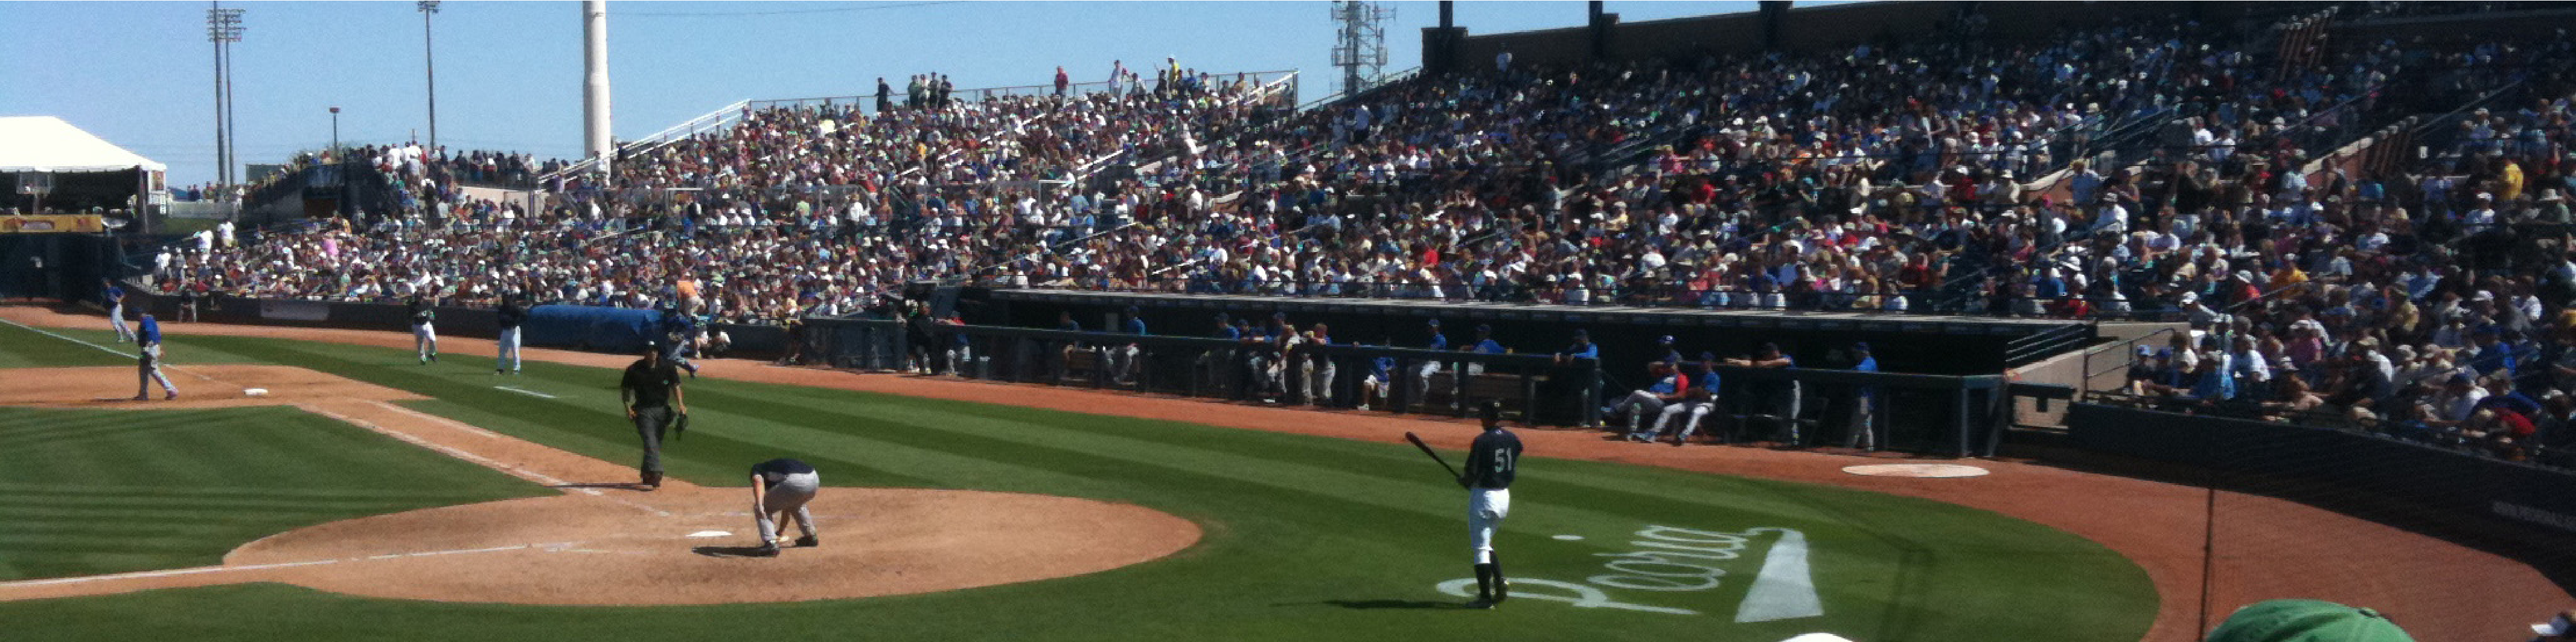
\includegraphics[width=\textwidth]{sampleteaser}
%   \caption{This is a teaser}
%   \label{fig:teaser}
% \end{teaserfigure}
% \end{verbatim}
%
%
% \DescribeMacro{\settopmatter}%
% Some information in the top matter is printed for certain journals
% or proceedings and suppressed for others.  You may override these
% defaults using the command \cs{settopmatter}\marg{settings}.  The
% settings and their meanings are listed in
% Table~\ref{tab:settopmatter}.  For example,
% \begin{verbatim}
% \settopmatter{printacmref=false, printccs=true, printfolios=true}
% \end{verbatim}
%
%
% \begin{table}
%   \centering
%   \caption{Settings for \cs{settopmatter} command}
%   \label{tab:settopmatter}
%   \begin{tabularx}{\textwidth}{llX}
%     \toprule
%     Parameter & Values & Meaning\\
%     \midrule
%     printccs & true/false & Whether to print CCS categories\\
%     printacmref & true/false & Whether to print ACM bibliographic
%     entry\\
%     printfolios & true/false & Whether to print page numbers (folios)\\
%     \bottomrule
%   \end{tabularx}
% \end{table}
%
%
% \DescribeMacro{\received}%
% The command \cs{received}\oarg{stage}\marg{date} sets the history of
% the publication.  The \oarg{stage} argument is optional; the default
% is |Received| for the first date and |revised| for the subsequent
% ones.  For example
% \begin{verbatim}
% \received{February 2007}
% \received[revised]{March 2009}
% \received[accepted]{June 2009}
% \end{verbatim}
%
%
% \DescribeMacro{\maketitle}%
% The macro \cs{maketitle} must be the last command in the top matter
% group:  i.e., it must follow the commands defined in this section.
%
%
% \DescribeMacro{\shortauthors}%
% \emph{After} the command \cs{maketitle} the macro \cs{shortauthors}
% stores the names of the authors for the running head.  You may
% redefine it if the list of author's name is too long, e.g.,
% \begin{verbatim}
% \maketitle
% \renewcommand{\shortauthors}{Zhou et al.}
% \end{verbatim}
%
%
%\subsection{Algorithms}
%\label{sec:ug_algorithms}
%
% There now several good packages for typesetting
% algorithms~\cite{Fiorio15, Brito09, Heinz15}, and the authors are
% now free to choose their favorite one.
%
%
%
%\subsection{Figures and tables}
%\label{sec:ug_floats}
%
% New ACM styles use the standard \LaTeX\ interface for figures and
% tables.  There are some important items to be aware of, however.
%
% \begin{enumerate}
% \item The captions for figures must be entered \emph{after} the
% figure bodies, and for the tables \emph{before} the table bodies.
% \item ACM uses the standard types for figures and types and adds
% several new ones.  In total there are follwing types:
% \begin{description}
% \item[figure, table:] a standard figure or table, taking full text
% width in one-column formats and one column in two-column formats.
% \item[figure*, table*] in two-column formats, a special figure or
% table taking full text width.
% \item[teaserfigure:] a special figure before \cs{maketitle}.
% \item[sidebar, marginfigure, margintable:] in the |sigchi-a| format,
%   special sidebars, tables and figures on the margin.
% \end{description}
%
% \item Accordingly, when scaling the images, one should use the
% following sizes:
% \begin{enumerate}
% \item For |figure| in one-column mode, |figure*| in two-column mode
%   or |teaserfigure|---\cs{textwidth} (in the one-column you can also
%   use \cs{columnwidth}, which coincides with \cs{textwidth} in this
%   case).
% \item For |figure| in two-column mode---\cs{columnwidth}.
% \item For |marginfigure|--\cs{marginparwidth}.
% \item For |figure*| in SIGCHI Extended
% abstracts---\cs{fulltextwidth}.
% \end{enumerate}
%
% \end{enumerate}
%
% It is strongly recommended to use the package booktabs~\cite{Fear05}
% and follow its main principles of typography with respect to tables:
% \begin{enumerate}
% \item Never, ever use vertical rules.
% \item Never use double rules.
% \end{enumerate}
% It is also a good idea not to overuse horizontal rules.
%
% For table \emph{footnotes} you have several options described in TeX
% FAQ~\cite{TeXFAQ}. The simplest one is to use \cs{minipage}
% environment:
% \begin{verbatim}
% \begin{table}
% \caption{Simulation Configuration}
% \label{tab:conf}
% \begin{minipage}{\columnwidth}
% \begin{center}
% \begin{tabular}{ll}
%   \toprule
%   TERRAIN\footnote{This is a table footnote. This is a
%     table footnote. This is a table footnote.}   &
%     (200\,m$\times$200\,m) Square\\
%   Node Number     & 289\\
%   Node Placement  & Uniform\\
%   Application     & Many-to-Many/Gossip CBR Streams\\
%   Payload Size    & 32 bytes\\
%   Routing Layer   & GF\\
%   MAC Layer       & CSMA/MMSN\\
%   Radio Layer     & RADIO-ACCNOISE\\
%   Radio Bandwidth & 250Kbps\\
%   Radio Range     & 20m--45m\\
%   \bottomrule
% \end{tabular}
% \end{center}
% \bigskip
% \footnotesize\emph{Source:} This is a table
%  sourcenote. This is a table sourcenote. This is a table
%  sourcenote.
%
%  \emph{Note:} This is a table footnote.
% \end{minipage}
% \end{table}
% \end{verbatim}
%
% \DescribeEnv{sidebar}%
% \DescribeEnv{marginfigure}%
% \DescribeEnv{margintable}%
% SIGCHI extended abstract extensively uses margin space.  The package
% provides three environments for this with option captions:
% \begin{description}
% \item[sidebar:] textual information on the margin
% \item[marginfigure:] a figure on the margin
% \item[margintable:] a table on the margin
% \end{description}
%
%
% Tables and figures (including margin tables and margin figures) are
% by default centered.  However, in some cases (for example, when you
% use several subimages per figure) you may need to override this
% decision.  A good way to do so is to put the contents into a
% \cs{minipage} of the width \cs{columnwidth}.  
%
%\subsection{Theorems}
%\label{sec:ug_theorems}
%
% ACM classes define two theorem styles and several pre-defined
% theorem environments:
% \begin{description}
% \item[acmplain:] this is  the style used for
% |theorem|,
% |conjecture|,
% |proposition|,
% |lemma|,
% |corollary|, and
% \item[acmdefinition:] this is the style used for |example| and
% |definition|.
% \end{description}
%
%
%
%
%
%\subsection{Online-only and offline-only material}
%\label{sec:ug_screen}
%
% \DescribeEnv{printonly}%
% \DescribeEnv{screenonly}%
% Some supplementary material in ACM publication is put online, but
% not in the printed version.  The text inside the environment
% |screenonly| will be typeset only when the option |screen| (see
% Section~\ref{sec:invocation}) is set to |true|.  Conversely, the
% text inside the environment |printonly| is typset only when this
% option is set to |false|.  For example
% \begin{verbatim}
% \section{Supplementary materials}
%
% \begin{printonly}
%   This section is included in the online version of the paper.
% \end{printonly}
%
% \begin{screenonly}
%   (The actual section).
% \end{screenonly}
% \end{verbatim}
%
% We use \textsl{comment} package for typesetting this code, so
% |\begin| and |\end| should start at the first positions of the lines
% of their own (no initial spaces etc.).
%
%\subsection{Note about anonymous mode}
%\label{sec:ug_anonymous}
%
% \DescribeEnv{anonsuppress}%
% When the option |anonymous| is selected, \TeX\ suppresses author
% information (including number of authors) for a blind review.
% However, sometimes the information identifying the authors may be
% present in the body of the paper
% \begin{verbatim}
% \begin{anonsuppress}
%   This is the continuation of the previous work by the author
%   \cite{prev1, prev2}.  
% \end{anonsuppress}
% \end{verbatim}
%
% As for |printonly| and |screenonly| environments,
% |\begin{anonsuppress}| and |\end{anonsuppress}| should start the
% line of their own (no leading or trailing spaces).  
% 
%\subsection{Acknowledgments}
%\label{sec:ug_acks}
%
% The traditional ``Acknowledgments'' section is conventionally used
% to thank persons and granting agencies for their help and support.
% However, there are several important considerations about this
% section.
%
% First, in the anonymous mode this section must be omitted: it gives
% too much information to the reviewers.  Second, the data about
% the grants is extracted and stored separately by the postprocessing
% software.  ACM classes provide facilities for both these tasks.
%
% \DescribeEnv{acks}%
% The environment |acks| starts an unnumbered section
% ``Acknowledgments'' unless the anonymous mode is chosen.  Put all
% thanks inside this environment.
%
% As for |printonly| and |screenonly| environments,
% |\begin{acks}| and |\end{acls}| should start the
% line of their own (no leading or trailing spaces).  

%
% \DescribeMacro{\grantsponsor}%
% \DescribeMacro{\grantnum}%
% All the financial support \emph{must} be listed using the commands
% \cs{grantsponsor} and \cs{grantnum}.  These commands tell the
% postprocessing software about the granting organization and the
% grant.  The format of the command is the following:
% \begin{quote}
%   \cs{grantsponsor}\marg{sponsorID}\marg{name}\marg{url}\\
%   \cs{grantnum}\oarg{url}\marg{sponsorID}\marg{number}.
% \end{quote}
% Here \marg{sponsorID} is the unique ID used to match grants to
% sponsors, \marg{name} is the name of the sponsor, \marg{url} is its
% URL, and \marg{number} is the grant number.  The \marg{sponsorID} of
% the \cs{grantnum} command must correspond to \cs{sponsorID} of a
% \cs{grantsponsor command}.  Some awards have their own web pages,
% which you can include using the optional argument of \cs{grantnum}
% command. 
%
% Example:
% \begin{verbatim}
% \begin{acks}
%   The authors would like to thank Dr. Yuhua Li for providing the
%   matlab code of  the \textit{BEPS} method. 
%
%   The authors would also like to thank the anonymous referees for
%   their valuable comments and helpful suggestions. The work is
%   supported by the \grantsponsor{GS501100001809}{National Natural
%   Science Foundation of
%   China}{http://dx.doi.org/10.13039/501100001809} under Grant
%   No.:~\grantnum{GS501100001809}{61273304}
%   and~\grantnum[http://www.nnsf.cn/youngscientsts]{GS501100001809}{Young 
%   Scientsts' Support Program}.
% \end{acks}
% \end{verbatim}
% 
%
%\subsection{Bibliography}
%\label{sec:ug_bibliography}
%
% ACM uses \textsl{natbib} package for formatting of referencing ant
% the style \path{ACM-Reference-Format.bst} for Bib\TeX\
% processing.  You may disable loading of \textsl{natbib} by using the
% option |natbib=false| in \cs{documentclass}.  However, it is not
% recommended, as well as the use of Bib\TeX\ styles other than
% \path{ACM-Reference-Format.bst}, and may delay the processing of the
% manuscript.  
% 
%
% \DescribeMacro{\citestyle}%
% If you use |natbib|, you can select one of two predefined sitation
% styles: the author-year format |acmauthoryear| or the numeric
% format |acmnumeric| using the command \cs{citestyle}, for example,
% \begin{verbatim}
% \citestyle{acmauthoryear}
% \end{verbatim}
% Note that numeric citations are the default mode for most formats.  
%  
% \DescribeMacro{\setcitestyle}%
% You may further customize
% \textsl{natbib} using \cs{setcitestyle} command, for example,
% \begin{verbatim}
% \setcitestyle{numbers,sort&compress}
% \end{verbatim}
%
% If you use |natbib|, then commands like \cs{citep} and
% \cs{citeauthor} are automatically supported.  The command
% \cs{shortcite} is the same as \cs{cite} in numerical mode, and cites
% the year in the author-date mode.
%
% There are several customized \BibTeX\ entries and fields in ACM
% style \path{ACM-Reference-Format.bst} you may want to be aware of.
%
% The style supports fields \path{doi} and \path{url}, for example,
% \begin{verbatim}
%  doi = "10.1145/1188913.1188915",
%  url = "http://ccrma.stanford.edu/~jos/bayes/bayes.pdf",
% \end{verbatim}
% 
% The style supports arXiv recommended fields \path{eprint} and
% (optionally) \path{primaryclass}, for example,
% \begin{verbatim}
%  eprint      = "960935712",
%  primaryclass = "cs",
% \end{verbatim}
% See the examples at \url{http://arxiv.org/hypertex/bibstyles/}.
%
% There are special entries \path{online}  and
% \path{game} for Web pages and games, for example,
% \begin{verbatim}
% @online{Thornburg01,
%  author = "Harry Thornburg",
%  year =   "2001",
%  title =  "Introduction to Bayesian Statistics",
%  url =    "http://ccrma.stanford.edu/~jos/bayes/bayes.html",
%  month =   mar,
%  lastaccessed = "March 2, 2005",
% }
% \end{verbatim}
% For these entries you can use the \path{lastaccessed} field to add
% the access date to the URL.
% 
% There are two ways to enter video and audio sources in the
% bibliograpy corresponding to two different possibilies.  For
% standalone sources available on WWW you can use an \path{online}
% entry, setting there \path{howpublished} field, for example,
% \begin{verbatim}
% @online{Obama08,
%  author = "Barack Obama",
%  year   = "2008",
%  title  = "A more perfect union",
%  howpublished  = "Video",
%  day 	  = "5",
%  url    = "http://video.google.com/videoplay?docid=6528042696351994555",
%  month  = mar,
%  lastaccessed = "March 21, 2008",
% }
% \end{verbatim}
% 
% For the sources available as attachments to conference proceedings
% and similar documents, you can use the usual \path{inproceedings}
% entry, again setting the \path{howpublished} field:
% \begin{verbatim}
% @Inproceedings{Novak03,
%  author =       "Dave Novak",
%  title =        "Solder man",
%  booktitle =    {ACM SIGGRAPH 2003 Video Review on Animation theater 
%                  Program},
%  year =         "2003",
%  publisher = 	 "ACM Press",
%  address = 	 "New York, NY",
%  pages =        "4",
%  month = 	 "March 21, 2008",
%  doi = 	 "99.9999/woot07-S422",
%  howpublished = "Video"
% }
% \end{verbatim}
% 
% Sometimes you need to cite a complete issue of a journal.  The entry
% \path{periodical} is intended for this:
% \begin{verbatim}
% @periodical{JCohen96,
%  key = 	 "Cohen",
%  editor =       "Jacques Cohen",
%  title =        "Special issue: Digital Libraries",
%  journal =      CACM,
%  volume =       "39",
%  number = 	 "11",
%  month =	 nov,
%  year = 	 "1996",
% }
%
% \end{verbatim}
% 
%
%\subsection{Colors}
%\label{sec:ug_colors}
%
% While printed ACM publications are usually black and white, screen
% mode allows the use of colors.  The ACM classes pre-define several
% colors according to~\cite{ACMIdentityStandards}:  |ACMBlue|,
% |ACMYellow|, |ACMOrange|, |ACMRed|, |ACMLightBlue|, |ACMGreen|,
% |ACMPurple|, |ACMDarkBlue|.  You can use them in the color
% assignments.
%
%
%\subsection{Other notable packages and typographic remarks}
%\label{sec:ug_other}
%
% Several other packages are recommended for specialized tasks.
%
% The package \textsl{subcaption}~\cite{Sommerfeldt13:Subcaption} is
% recommended for complex figures with several subplots or subfigures
% that require separate subcaptioning.  The packages
% \textsl{nomencl}~\cite{Nomencl} and
% \textsl{glossaries}~\cite{Talbot16:Glossaries} can be used for the
% automatic creation of the lists of symbols and concepts used.  
%
%
% By default |acmart| prevents all widows and orphans (i.e. lonely
% lines at the beginning and the end of the page) and hyphenation at
% the end of the page.  This is done by rather strict settings
% \begin{verbatim}
% \widowpenalty=10000
% \clubpenalty=10000
% \brokenpenalty=10000
% \end{verbatim}
% However, this may lead to frustrating results when the authors must
% obey a page limit.  Setting these penalties to smaller values may
% help if you absolutely need to.
%
% Another problem might be the too strict line breaking rules.  Again,
% a strategically placed \cs{sloppy} command or putting the
% problematic paragraph inside \texttt{sloppypar} environment might
% help---but beware the results might be, well, sloppy.
%
%
%
% \StopEventually{
% \clearpage
% \bibliography{acmart}
% \bibliographystyle{unsrt}}
%
% \clearpage
%
%
%\section{Implementation}
%\label{sec:impl}
%
%\subsection{Identification}
%\label{sec:ident}
%
% We start with the declaration who we are.  Most |.dtx| files put
% driver code in a separate driver file |.drv|.  We roll this code into the
% main file, and use the pseudo-guard |<gobble>| for it.
%    \begin{macrocode}
%<class>\NeedsTeXFormat{LaTeX2e}
%<*gobble>
\ProvidesFile{acmart.dtx}
%</gobble>
%<class>\ProvidesClass{acmart}
[2017/01/07 v1.28 Typesetting articles for Association of
Computing Machinery]
%    \end{macrocode}
%
% \changes{v1.00}{2016/04/14}{First released version}
% \changes{v1.01}{2016/04/18}{Defined ACM colors}
% \changes{v1.01}{2016/04/18}{Changed hyperref colors in screen mode
% (closes \url{https://github.com/borisveytsman/acmart/issues/1})}
% \changes{v1.01}{2016/04/18}{Set headheight to 1pc for all formats
% (closes \url{https://github.com/borisveytsman/acmart/issues/5})}
% \changes{v1.02}{2016/04/21}{Documentation changes
% (closes \url{https://github.com/borisveytsman/acmart/issues/13})}
% \changes{v1.02}{2016/04/21}{Added TOPS and TSC
% (closes \url{https://github.com/borisveytsman/acmart/issues/12})}
% \changes{v1.03}{2016/04/22}{Added authorversion option
% (closes \url{https://github.com/borisveytsman/acmart/issues/9})}
% \changes{v1.03}{2016/04/22}{Added anonsuppress environment}
% \changes{v1.04}{2016/04/26}{Updated bibliography for siggraph}
% \changes{v1.05}{2016/04/27}{Patched \cs{setcitestyle} command;
% closes \url{https://github.com/borisveytsman/acmart/issues/19}}
% \changes{v1.05}{2016/04/27}{Added processing doi numbers for
% acmsiggraph and doi numbers for sigproc.bib}
% \changes{v1.08}{2016/05/13}{SIGPLAN reformatting by Matthew Fluet}
% \changes{v1.08}{2016/05/13}{Typos corrected (Tobias Pape)}
% \changes{v1.09}{2016/05/18}{Revert SIGPLAN caption rules}
% \changes{v1.11}{2016/05/27}{Customization of ACM theorem styles and
% proof environment by Matthew Fluet}
% \changes{v1.12}{2016/05/30}{Documentation updates}
% \changes{v1.14}{2016/06/09}{\cs{citestyle} updates (Matthew Fluet)}
% \changes{v1.16}{2016/07/07}{Formatting header/footer (Matthew
% Fluet)}
% \changes{v1.18}{2016/07/10}{Natbib is now the default for all
% formats} 
% \changes{v1.19}{2016/07/28}{Include 'Abstract', 'Acknowledgements',
% and 'References' in PDF bookmarks (Matthew Fluet)}
% \changes{v1.20}{2016/08/06}{Bug fixes for bst}
% \changes{v1.22}{2016/09/25}{More bibliography changes for Aptara}
% \changes{v1.23}{2016/11/04}{Add PACMPL journal option}
% \changes{v1.26}{2016/12/24}{Corrected \cs{shortcite} bug}
% \changes{v1.26}{2016/12/24}{Documentation typos fixed (thanks to
% Stephen Spencer)} 
%
%
% And the driver code:
%    \begin{macrocode}
%<*gobble>
\documentclass{ltxdoc}
\usepackage{array,booktabs,amsmath,graphicx,fancyvrb,tabularx}
\usepackage[tt=false]{libertine}
\usepackage[varqu]{zi4}
\usepackage[libertine]{newtxmath}
\usepackage[tableposition=top]{caption}
\usepackage{hypdoc}
\PageIndex
\CodelineIndex
\RecordChanges
\EnableCrossrefs
\begin{document}
  \DocInput{acmart.dtx}
\end{document}
%</gobble>
%<*class>
\def\@classname{acmart}
%    \end{macrocode}
%
% \subsection{Options}
% \label{sec:options}
%
% We need |xkeyval| since some of our options may have values:
%    \begin{macrocode}
\RequirePackage{xkeyval}
%    \end{macrocode}
%
% \begin{macro}{format}
%   The possible formats
%    \begin{macrocode}
\define@choicekey*+{acmart.cls}{format}[\ACM@format\ACM@format@nr]{%
  manuscript, acmsmall, acmlarge, acmtog, sigconf, siggraph,
  sigplan, sigchi, sigchi-a}[manuscript]{}{%
  \ClassError{\@classname}{The option format must be manuscript,
    acmsmall, acmlarge, acmtog, sigconf, siggraph,
    sigplan, sigchi or sigchi-a}}
\def\@DeclareACMFormat#1{\DeclareOptionX{#1}{\setkeys{acmart.cls}{format=#1}}}
\@DeclareACMFormat{manuscript}
\@DeclareACMFormat{acmsmall}
\@DeclareACMFormat{acmlarge}
\@DeclareACMFormat{acmtog}
\@DeclareACMFormat{sigconf}
\@DeclareACMFormat{siggraph}
\@DeclareACMFormat{sigplan}
\@DeclareACMFormat{sigchi}
\@DeclareACMFormat{sigchi-a}
\ExecuteOptionsX{format}
%    \end{macrocode}
%
% \end{macro}
%
% \begin{macro}{\if@ACM@screen}
%   Whether we use screen mode
%    \begin{macrocode}
\define@boolkey+{acmart.cls}[@ACM@]{screen}[true]{%
  \if@ACM@screen
    \PackageInfo{\@classname}{Using screen mode}%
  \else
    \PackageInfo{\@classname}{Not using screen mode}%
  \fi}{\PackageError{\@classname}{Option screen can be either true or
    false}}
\ExecuteOptionsX{screen=false}
%    \end{macrocode}
%
% \end{macro}
%
%
% \begin{macro}{\if@ACM@review}
%   Whether we use review mode
%    \begin{macrocode}
\define@boolkey+{acmart.cls}[@ACM@]{review}[true]{%
  \if@ACM@review
    \PackageInfo{\@classname}{Using review mode}%
  \else
    \PackageInfo{\@classname}{Not using review mode}%
  \fi}{\PackageError{\@classname}{Option review can be either true or
    false}}
\ExecuteOptionsX{review=false}
%    \end{macrocode}
%
% \end{macro}
%
% \begin{macro}{\if@ACM@authorversion}
% \changes{v1.03}{2016/04/22}{Added macro}
%   Whether we use author's version
%    \begin{macrocode}
\define@boolkey+{acmart.cls}[@ACM@]{authorversion}[true]{%
  \if@ACM@authorversion
    \PackageInfo{\@classname}{Using authorversion mode}%
  \else
    \PackageInfo{\@classname}{Not using authorversion mode}%
  \fi}{\PackageError{\@classname}{Option authorversion can be either true or
    false}}
\ExecuteOptionsX{authorversion=false}
%    \end{macrocode}
%
% \end{macro}
%
%
% \begin{macro}{\if@ACM@natbib@override}
% \changes{v1.12}{2016/05/30}{Added macro}
%   Whether to override the format decision about \textsl{natbib}
%    \begin{macrocode}
\newif\if@ACM@natbib@override
\@ACM@natbib@overridefalse
%    \end{macrocode}
%   
% \end{macro}
%
% \begin{macro}{\if@ACM@natbib}
%   Whether we use natbib mode
%    \begin{macrocode}
\define@boolkey+{acmart.cls}[@ACM@]{natbib}[true]{%
  \@ACM@natbib@overridetrue
  \if@ACM@natbib
    \PackageInfo{\@classname}{Explicitly selecting natbib mode}%
  \else
    \PackageInfo{\@classname}{Explicitly deselecting natbib mode}%
  \fi}{\PackageError{\@classname}{Option natbib can be either true or
    false}}
%    \end{macrocode}
%
% \end{macro}
%
%
% \begin{macro}{\if@ACM@anonymous}
%   Whether we use anonymous mode
%    \begin{macrocode}
\define@boolkey+{acmart.cls}[@ACM@]{anonymous}[true]{%
  \if@ACM@anonymous
    \PackageInfo{\@classname}{Using anonymous mode}%
  \else
    \PackageInfo{\@classname}{Not using anonymous mode}%
  \fi}{\PackageError{\@classname}{Option anonymous can be either true or
    false}}
\ExecuteOptionsX{anonymous=false}
%    \end{macrocode}
%
% \end{macro}
%
% \begin{macro}{\ACM@fontsize}
%   The font size to pass to the base class
%    \begin{macrocode}
\def\ACM@fontsize{}
\DeclareOptionX{9pt}{\edef\ACM@fontsize{\CurrentOption}}
\DeclareOptionX{10pt}{\edef\ACM@fontsize{\CurrentOption}}
\DeclareOptionX{11pt}{\edef\ACM@fontsize{\CurrentOption}}
\DeclareOptionX{12pt}{\edef\ACM@fontsize{\CurrentOption}}
%    \end{macrocode}
%
% \end{macro}
%
%
% \changes{v1.01}{2016/04/18}{Explicitly put draft option
% (closes \url{https://github.com/borisveytsman/acmart/issues/4})}
%
%    \begin{macrocode}
\DeclareOptionX{draft}{\PassOptionsToClass{\CurrentOption}{amsart}}
\DeclareOptionX{*}{\PassOptionsToClass{\CurrentOption}{amsart}}
\ProcessOptionsX
\ClassInfo{\@classname}{Using format \ACM@format, number \ACM@format@nr}
%    \end{macrocode}
%
%
%
%\subsection{Setting switches}
%\label{sec:switches}
%
% \begin{macro}{\if@ACM@manuscript}
%   Whether we use manuscript mode
%    \begin{macrocode}
\newif\if@ACM@manuscript
%    \end{macrocode}
%
% \end{macro}
%
% \begin{macro}{\if@ACM@journal}
%   There are two kinds of publications: journals and books
%    \begin{macrocode}
\newif\if@ACM@journal
%    \end{macrocode}
%
% \end{macro}
%
% \begin{macro}{\if@ACM@sigchiamode}
%   The formatting of SIGCHI abstracts is quite unusual.  We have a
%   special switch for them.
%    \begin{macrocode}
\newif\if@ACM@sigchiamode
%    \end{macrocode}
%
% \end{macro}
%
%
% Setting up switches
%    \begin{macrocode}
\ifnum\ACM@format@nr=0\relax
  \@ACM@manuscripttrue
\else
  \@ACM@manuscriptfalse
\fi
\@ACM@sigchiamodefalse
\ifcase\ACM@format@nr
\relax % manuscript
  \@ACM@journaltrue
\or % acmsmall
  \@ACM@journaltrue
\or % acmlarge
  \@ACM@journaltrue
\or % acmtog
  \@ACM@journaltrue
\or % sigconf
  \@ACM@journalfalse
\or % siggraph
  \@ACM@journalfalse
 \or % sigplan
  \@ACM@journalfalse
 \or % sigchi
  \@ACM@journalfalse
\or % sigchi-a
  \@ACM@journalfalse
  \@ACM@sigchiamodetrue
\fi
%    \end{macrocode}
%
% A format sets up \cs{if@ACM@natbib} only if
% \cs{@ACM@natbib@override} is false (i.e. user did \emph{not}
% overrode format's selection):
%    \begin{macrocode}
\if@ACM@natbib@override\else
    \@ACM@natbibtrue
\fi
%    \end{macrocode}
% 
%
%\subsection{Loading base class and package}
%\label{sec:loading}
%
% \changes{v1.13}{2016/06/06}{Increased font size for ACM Large}
%
%
% At this point we either have \cs{ACM@fontsize}, or use defaults
%    \begin{macrocode}
\ifx\ACM@fontsize\@empty
  \ifcase\ACM@format@nr
  \relax % manuscript
    \def\ACM@fontsize{9pt}%
  \or % acmsmall
    \def\ACM@fontsize{10pt}%
  \or % acmlarge
    \def\ACM@fontsize{10pt}%
  \or % acmtog
    \def\ACM@fontsize{9pt}%
  \or % sigconf
    \def\ACM@fontsize{9pt}%
  \or % siggraph
    \def\ACM@fontsize{9pt}%
   \or % sigplan
    \def\ACM@fontsize{9pt}%
   \or % sigchi
    \def\ACM@fontsize{10pt}%
  \or % sigchi-a
    \def\ACM@fontsize{10pt}%
  \fi
\fi
\ClassInfo{\@classname}{Using fontsize \ACM@fontsize}
\LoadClass[\ACM@fontsize, reqno]{amsart}
\RequirePackage{microtype}
%    \end{macrocode}
%
%
% We need |totpages| package to calculate the number of pages
%    \begin{macrocode}
\RequirePackage{totpages}
%    \end{macrocode}
%
% The |amsmath| \cs{collect@body} is defined using \cs{def}.  We load
% |environ| to access the \cs{long} version of the command
%    \begin{macrocode}
\RequirePackage{environ}
%    \end{macrocode}
%
% We use |setspace| for doublespacing
%    \begin{macrocode}
\if@ACM@manuscript
\RequirePackage{setspace}
\onehalfspacing
\fi
%    \end{macrocode}
%
% \changes{v1.19}{2016/07/28}{Include 'References' in PDF bookmarks
% (Matthew Fluet)}
% \changes{v1.14}{2016/06/09}{Patched \cs{citestyle}}
% Citations.  We patch \cs{setcitestyle} to allow, e.g.,
% \cs{setcitestyle}|{sort}| and \cs{setcitestyle}|{nosort}|.  We patch
% \cs{citestyle} to warn about undefined citation styles.
%    \begin{macrocode}
\if@ACM@natbib
  \RequirePackage{natbib}
  \renewcommand{\bibsection}{%
     \section*{\refname}%
     \phantomsection\addcontentsline{toc}{section}{\refname}%
  }
  \renewcommand{\bibfont}{\bibliofont}
  \renewcommand\setcitestyle[1]{
  \@for\@tempa:=#1\do
  {\def\@tempb{round}\ifx\@tempa\@tempb
     \renewcommand\NAT@open{(}\renewcommand\NAT@close{)}\fi
   \def\@tempb{square}\ifx\@tempa\@tempb
     \renewcommand\NAT@open{[}\renewcommand\NAT@close{]}\fi
   \def\@tempb{angle}\ifx\@tempa\@tempb
     \renewcommand\NAT@open{$<$}\renewcommand\NAT@close{$>$}\fi
   \def\@tempb{curly}\ifx\@tempa\@tempb
     \renewcommand\NAT@open{\{}\renewcommand\NAT@close{\}}\fi
   \def\@tempb{semicolon}\ifx\@tempa\@tempb
     \renewcommand\NAT@sep{;}\fi
   \def\@tempb{colon}\ifx\@tempa\@tempb
     \renewcommand\NAT@sep{;}\fi
   \def\@tempb{comma}\ifx\@tempa\@tempb
     \renewcommand\NAT@sep{,}\fi
   \def\@tempb{authoryear}\ifx\@tempa\@tempb
     \NAT@numbersfalse\fi
   \def\@tempb{numbers}\ifx\@tempa\@tempb
     \NAT@numberstrue\NAT@superfalse\fi
   \def\@tempb{super}\ifx\@tempa\@tempb
     \NAT@numberstrue\NAT@supertrue\fi
   \def\@tempb{nobibstyle}\ifx\@tempa\@tempb
     \let\bibstyle=\@gobble\fi
   \def\@tempb{bibstyle}\ifx\@tempa\@tempb
     \let\bibstyle=\@citestyle\fi
   \def\@tempb{sort}\ifx\@tempa\@tempb
     \def\NAT@sort{\@ne}\fi
   \def\@tempb{nosort}\ifx\@tempa\@tempb
     \def\NAT@sort{\z@}\fi
   \def\@tempb{compress}\ifx\@tempa\@tempb
     \def\NAT@cmprs{\@ne}\fi
   \def\@tempb{nocompress}\ifx\@tempa\@tempb
     \def\NAT@cmprs{\@z}\fi
   \def\@tempb{sort&compress}\ifx\@tempa\@tempb
     \def\NAT@sort{\@ne}\def\NAT@cmprs{\@ne}\fi
   \def\@tempb{mcite}\ifx\@tempa\@tempb
     \let\NAT@merge\@ne\fi
   \def\@tempb{merge}\ifx\@tempa\@tempb
     \@ifnum{\NAT@merge<\tw@}{\let\NAT@merge\tw@}{}\fi
   \def\@tempb{elide}\ifx\@tempa\@tempb
     \@ifnum{\NAT@merge<\thr@@}{\let\NAT@merge\thr@@}{}\fi
   \def\@tempb{longnamesfirst}\ifx\@tempa\@tempb
     \NAT@longnamestrue\fi
   \def\@tempb{nonamebreak}\ifx\@tempa\@tempb
     \def\NAT@nmfmt#1{\mbox{\NAT@up#1}}\fi
   \expandafter\NAT@find@eq\@tempa=\relax\@nil
   \if\@tempc\relax\else
     \expandafter\NAT@rem@eq\@tempc
     \def\@tempb{open}\ifx\@tempa\@tempb
      \xdef\NAT@open{\@tempc}\fi
     \def\@tempb{close}\ifx\@tempa\@tempb
      \xdef\NAT@close{\@tempc}\fi
     \def\@tempb{aysep}\ifx\@tempa\@tempb
      \xdef\NAT@aysep{\@tempc}\fi
     \def\@tempb{yysep}\ifx\@tempa\@tempb
      \xdef\NAT@yrsep{\@tempc}\fi
     \def\@tempb{notesep}\ifx\@tempa\@tempb
      \xdef\NAT@cmt{\@tempc}\fi
     \def\@tempb{citesep}\ifx\@tempa\@tempb
      \xdef\NAT@sep{\@tempc}\fi
   \fi
  }%
  \NAT@@setcites
  }
  \renewcommand\citestyle[1]{%
    \ifcsname bibstyle@#1\endcsname%
    \csname bibstyle@#1\endcsname\let\bibstyle\@gobble%
    \else%
    \@latex@error{Undefined `#1' citestyle}%
    \fi
  }%
\fi
%    \end{macrocode}
%
% \begin{macro}{\bibstyle@acmauthoryear}
% \changes{v1.13}{2016/06/06}{Added macro}
% \changes{v1.14}{2016/06/09}{Moved def of \cs{bibstyle@acmauthoryear}
%   before use}
%   The default author-year format:
%    \begin{macrocode}
\newcommand{\bibstyle@acmauthoryear}{%
  \setcitestyle{%
    authoryear,%
    open={(},close={)},citesep={;},%
    aysep={},yysep={,},%
    notesep={, }}}
%    \end{macrocode}
%
% \end{macro}
%
% \begin{macro}{\bibstyle@acmnumeric}
% \changes{v1.13}{2016/06/06}{Added macro}
% \changes{v1.14}{2016/06/09}{Moved def of \cs{bibstyle@numeric}
%   before use}
%   The default numeric format:
%    \begin{macrocode}
\newcommand{\bibstyle@acmnumeric}{%
  \setcitestyle{%
    numbers,sort&compress,%
    open={[},close={]},citesep={,},%
    notesep={, }}}
%    \end{macrocode}
%
% \end{macro}
%
% \changes{v1.28}{2017/01/07}{Corrected option natbib behavior}
% The default is numeric:
%    \begin{macrocode}
\if@ACM@natbib
\citestyle{acmnumeric}
\fi
%    \end{macrocode}
% 
%
% Before we call |hyperref|, we redefine \cs{startsection} commands to
% their \LaTeX\ defaults, since |amsart| ones are too AMS-specific.
% We need to do this early since we want |hyperref| to have a chance
% to redefine them again:
%    \begin{macrocode}
\def\@startsection#1#2#3#4#5#6{%
  \if@noskipsec \leavevmode \fi
  \par
  \@tempskipa #4\relax
  \@afterindenttrue
  \ifdim \@tempskipa <\z@
    \@tempskipa -\@tempskipa \@afterindentfalse
  \fi
  \if@nobreak
    \everypar{}%
  \else
    \addpenalty\@secpenalty\addvspace\@tempskipa
  \fi
  \@ifstar
    {\@ssect{#3}{#4}{#5}{#6}}%
    {\@dblarg{\@sect{#1}{#2}{#3}{#4}{#5}{#6}}}}
\def\@sect#1#2#3#4#5#6[#7]#8{%
  \ifnum #2>\c@secnumdepth
    \let\@svsec\@empty
  \else
    \refstepcounter{#1}%
    \protected@edef\@svsec{\@seccntformat{#1}\relax}%
  \fi
  \@tempskipa #5\relax
  \ifdim \@tempskipa>\z@
    \begingroup
      #6{%
        \@hangfrom{\hskip #3\relax\@svsec}%
          \interlinepenalty \@M #8\@@par}%
    \endgroup
    \csname #1mark\endcsname{#7}%
    \addcontentsline{toc}{#1}{%
      \ifnum #2>\c@secnumdepth \else
        \protect\numberline{\csname the#1\endcsname}%
      \fi
      #7}%
  \else
    \def\@svsechd{%
      #6{\hskip #3\relax
      \@svsec #8}%
      \csname #1mark\endcsname{#7}%
      \addcontentsline{toc}{#1}{%
        \ifnum #2>\c@secnumdepth \else
          \protect\numberline{\csname the#1\endcsname}%
        \fi
        #7}}%
  \fi
  \@xsect{#5}}
\def\@xsect#1{%
  \@tempskipa #1\relax
  \ifdim \@tempskipa>\z@
    \par \nobreak
    \vskip \@tempskipa
    \@afterheading
  \else
    \@nobreakfalse
    \global\@noskipsectrue
    \everypar{%
      \if@noskipsec
        \global\@noskipsecfalse
       {\setbox\z@\lastbox}%
        \clubpenalty\@M
        \begingroup \@svsechd \endgroup
        \unskip
        \@tempskipa #1\relax
        \hskip -\@tempskipa
      \else
        \clubpenalty \@clubpenalty
        \everypar{}%
      \fi}%
  \fi
  \ignorespaces}
\def\@seccntformat#1{\csname the#1\endcsname\quad}
\def\@ssect#1#2#3#4#5{%
  \@tempskipa #3\relax
  \ifdim \@tempskipa>\z@
    \begingroup
      #4{%
        \@hangfrom{\hskip #1}%
          \interlinepenalty \@M #5\@@par}%
    \endgroup
  \else
    \def\@svsechd{#4{\hskip #1\relax #5}}%
  \fi
  \@xsect{#3}}
%    \end{macrocode}
%
%
% And |hyperref|
% \changes{v1.28}{2017/01/07}{Got rid of warnings in pdf keywords}
%    \begin{macrocode}
\let\@footnotemark@nolink\@footnotemark
\let\@footnotetext@nolink\@footnotetext
\RequirePackage[bookmarksnumbered,unicode]{hyperref}
\pdfstringdefDisableCommands{%
  \def\unskip{}
  \def\textbullet{- }
  \def\textrightarrow{ -> }
  \def\footnotemark{}
}
\urlstyle{rm}
\ifcase\ACM@format@nr
\relax % manuscript
\or % acmsmall
\or % acmlarge
\or % acmtog
\or % sigconf
\or % siggraph
\or % sigplan
  \urlstyle{sf}
\or % sigchi
\or % sigchi-a
  \urlstyle{sf}
\fi
\if@ACM@screen
  \hypersetup{colorlinks,
    linkcolor=ACMRed,
    citecolor=ACMPurple,
    urlcolor=ACMDarkBlue,
    filecolor=ACMDarkBlue}
\else
  \hypersetup{hidelinks}
\fi
%    \end{macrocode}
%
% Bibliography mangling. 
%    \begin{macrocode}
\if@ACM@natbib
  \let\citeN\cite
  \let\cite\citep
  \let\citeANP\citeauthor
  \let\citeNN\citeyearpar
  \let\citeyearNP\citeyear
  \let\citeyear\citeyearpar
  \let\citeNP\citealt
  \DeclareRobustCommand\citeA
     {\begingroup\NAT@swafalse
       \let\NAT@ctype\@ne\NAT@partrue\NAT@fullfalse\NAT@open\NAT@citetp}%
  \providecommand\newblock{}%
\else
  \providecommand\citename[1]{#1}
\fi
\def\shortcite#1{\ifNAT@numbers\cite{#1}\else\citeyear{#1}\fi}
%    \end{macrocode}
%
%
% \begin{macro}{\bibliographystyle}
% \changes{v1.13}{2016/06/06}{Redefined macro}
%   Amsart redefines \cs{bibliographystyle} since it prefers AMS
%   bibliography.  We turn it back to \LaTeX\ definition:
%    \begin{macrocode}
\def\bibliographystyle#1{%
  \ifx\@begindocumenthook\@undefined\else
    \expandafter\AtBeginDocument
  \fi
    {\if@filesw
       \immediate\write\@auxout{\string\bibstyle{#1}}%
     \fi}}
%    \end{macrocode}
%   
% \end{macro}
%
%
% Graphics and color
%    \begin{macrocode}
\RequirePackage{graphicx, xcolor}
%    \end{macrocode}
%
% We define ACM colors according to~\cite{ACMIdentityStandards}:
%    \begin{macrocode}
\definecolor[named]{ACMBlue}{cmyk}{1,0.1,0,0.1}
\definecolor[named]{ACMYellow}{cmyk}{0,0.16,1,0}
\definecolor[named]{ACMOrange}{cmyk}{0,0.42,1,0.01}
\definecolor[named]{ACMRed}{cmyk}{0,0.90,0.86,0}
\definecolor[named]{ACMLightBlue}{cmyk}{0.49,0.01,0,0}
\definecolor[named]{ACMGreen}{cmyk}{0.20,0,1,0.19}
\definecolor[named]{ACMPurple}{cmyk}{0.55,1,0,0.15}
\definecolor[named]{ACMDarkBlue}{cmyk}{1,0.58,0,0.21}
%    \end{macrocode}
% 
%
%\subsection{Paper size and paragraphing}
%\label{sec:paper}
%
% \changes{v1.17}{2016/07/07}{Slightly decreased margins for sigs}
% We use |geometry| for dimensions
%    \begin{macrocode}
\RequirePackage{geometry}
\ifcase\ACM@format@nr
\relax % manuscript
   \geometry{letterpaper,head=1pc}%
\or % acmsmall
   \geometry{twoside=true,
     includeheadfoot, head=1pc, foot=2pc,
     paperwidth=6.75in, paperheight=10in,
     top=58pt, bottom=44pt, inner=46pt, outer=46pt
   }%
\or % acmlarge
   \geometry{twoside=true, head=1pc, foot=2pc,
     paperwidth=8.5in, paperheight=11in,
     includeheadfoot,
     top=78pt, bottom=114pt, inner=81pt, outer=81pt
     }%
\or % acmtog
   \geometry{twoside=true, head=1pc, foot=2pc,
     paperwidth=8.5in, paperheight=11in,
     includeheadfoot, columnsep=24pt,
     top=52pt, bottom=75pt, inner=52pt, outer=52pt
     }%
\or % sigconf
   \geometry{twoside=true, head=1pc,
     paperwidth=8.5in, paperheight=11in,
     includeheadfoot, columnsep=2pc,
     top=57pt, bottom=73pt, inner=54pt, outer=54pt
     }%
\or % siggraph
   \geometry{twoside=true, head=1pc,
     paperwidth=8.5in, paperheight=11in,
     includeheadfoot, columnsep=2pc,
     top=57pt, bottom=73pt, inner=54pt, outer=54pt
     }%
\or % sigplan
   \geometry{twoside=true, head=1pc,
     paperwidth=8.5in, paperheight=11in,
     includeheadfoot=false, columnsep=2pc,
     top=1in, bottom=1in, inner=0.75in, outer=0.75in
     }%
\or % sigchi
   \geometry{twoside=true, head=1pc,
     paperwidth=8.5in, paperheight=11in,
     includeheadfoot, columnsep=2pc,
     top=66pt, bottom=73pt, inner=54pt, outer=54pt
     }%
\or % sigchi-a
   \geometry{twoside=false, head=1pc,
     paperwidth=11in, paperheight=8.5in,
     includeheadfoot, marginparsep=72pt,
     marginparwidth=170pt, columnsep=20pt,
     top=72pt, bottom=72pt, left=314pt, right=72pt
     }%
     \@mparswitchfalse
     \reversemarginpar
\fi
%    \end{macrocode}
%
%
% \begin{macro}{\parindent}
% \begin{macro}{\parskip}
%   Paragraphing
%    \begin{macrocode}
\setlength\parindent{10\p@}
\setlength\parskip{\z@}
\ifcase\ACM@format@nr
\relax % manuscript
\or % acmsmall
\or % acmlarge
\or % acmtog
  \setlength\parindent{9\p@}%
\or % sigconf
\or % siggraph
\or % sigplan
\or % sigchi
\or % sigchi-a
\fi
%    \end{macrocode}
%
% \end{macro}
% \end{macro}
%
% Footnotes require some consideration.  We have several layers of
% footnotes:  frontmatter footnotes, ``regular'' footnotes and the
% special insert for bibstrip.  In the old ACM classes bibstrip was a
% \cs{@float}.  The problem with floats is that they tend to, well,
% float---and we want the guarantee they stay.  
%
% We use \textsl{manyfoot} for layered footnotes instead.
%
% \begin{macro}{\copyrightpermissionfootnoterule}
% \changes{v1.12}{2016/05/30}{Added macro}
%   This is the footnote rule that separates bibstrip from the rest of
%   the paper.  It is a full width rule.
%    \begin{macrocode}
\def\copyrightpermissionfootnoterule{\kern-3\p@
  \hrule \@width \columnwidth \kern 2.6\p@}
%    \end{macrocode}
% \end{macro}
%
%    \begin{macrocode}
\RequirePackage{manyfoot}
\SelectFootnoteRule[2]{copyrightpermission}
\DeclareNewFootnote{copyrightpermission}
%    \end{macrocode}
% 
%
% \begin{macro}{\footnoterule}
% \changes{v1.12}{2016/05/30}{Made shorter}
%   Tschichold's rules:
%    \begin{macrocode}
\def\footnoterule{\kern-3\p@
  \hrule \@width 4pc \kern 2.6\p@}
%    \end{macrocode}
%
% \end{macro}
%
% \begin{macro}{\endminipage}
%   We do not use footnote rules in minipages
%    \begin{macrocode}
\def\endminipage{%
    \par
    \unskip
    \ifvoid\@mpfootins\else
      \vskip\skip\@mpfootins
      \normalcolor
      \unvbox\@mpfootins
    \fi
    \@minipagefalse   %% added 24 May 89
  \color@endgroup
  \egroup
  \expandafter\@iiiparbox\@mpargs{\unvbox\@tempboxa}}
%    \end{macrocode}
%
% \end{macro}
%
% \begin{macro}{\@makefntext}
%   We do note use indentation for footnotes
%    \begin{macrocode}
\def\@makefntext{\noindent\@makefnmark}
%    \end{macrocode}
%
% \end{macro}
%
% \begin{macro}{\@footnotetext}
%   In sigchi-a mode our footnotes are on the margins!
%    \begin{macrocode}
\if@ACM@sigchiamode
\long\def\@footnotetext#1{\marginpar{%
    \reset@font\small
    \interlinepenalty\interfootnotelinepenalty
    \protected@edef\@currentlabel{%
       \csname p@footnote\endcsname\@thefnmark
    }%
    \color@begingroup
      \@makefntext{%
        \rule\z@\footnotesep\ignorespaces#1\@finalstrut\strutbox}%
    \color@endgroup}}%
\fi
%    \end{macrocode}
%
% \end{macro}
%
% \begin{macro}{\@mpfootnotetext}
% \changes{v1.13}{2016/06/06}{Made minipage footnotes centered}
%   We want the footnotes in minipages centered:
%    \begin{macrocode}
\long\def\@mpfootnotetext#1{%
  \global\setbox\@mpfootins\vbox{%
    \unvbox\@mpfootins
    \reset@font\footnotesize
    \hsize\columnwidth
    \@parboxrestore
    \protected@edef\@currentlabel
         {\csname p@mpfootnote\endcsname\@thefnmark}%
    \color@begingroup\centering
      \@makefntext{%
        \rule\z@\footnotesep\ignorespaces#1\@finalstrut\strutbox}%
    \color@endgroup}}
%    \end{macrocode}
%   
% \end{macro}
% 
% \begin{macro}{\@makefnmark}
% \changes{v1.17}{2016/067/09}{Redefined}
%   AMS classes use a buggy definition of \cs{makefnmark}.  We revert
%   to the standard one.
%    \begin{macrocode}
\def\@makefnmark{\hbox{\@textsuperscript{\normalfont\@thefnmark}}}
%    \end{macrocode}
%   
% \end{macro}
%
%\subsection{Fonts}
%\label{sec:fonts}
%
% \changes{v1.12}{2016/05/30}{Added graceful behavior when libertine
% fonts are absent}%
%
% \begin{macro}{\if@ACM@newfonts}
% \changes{v1.12}{2016/05/30}{Added macro}%
%   Whether we load the new fonts
%    \begin{macrocode}
\newif\if@ACM@newfonts
\@ACM@newfontstrue
\IfFileExists{libertine.sty}{}{\ClassWarning{\@classname}{You do not
    have libertine package installed.  Please upgrade your 
    TeX}\@ACM@newfontsfalse}
\IfFileExists{zi4.sty}{}{\ClassWarning{\@classname}{You do not
    have zi4 package installed.  Please upgrade your TeX}\@ACM@newfontsfalse}
\IfFileExists{newtxmath.sty}{}{\ClassWarning{\@classname}{You do not
    have newtxmath package installed.  Please upgrade your
    TeX}\@ACM@newfontsfalse} 
%    \end{macrocode}
%   
% \end{macro}
% 
% We use Libertine throughout.
%    \begin{macrocode}
\if@ACM@newfonts
\RequirePackage[tt=false]{libertine}
\RequirePackage[varqu]{zi4}
\RequirePackage[libertine]{newtxmath}
\fi
%    \end{macrocode}
%
% The SIGCHI extended abstracts are sans serif:
%    \begin{macrocode}
\if@ACM@sigchiamode
  \renewcommand{\familydefault}{\sfdefault}
\fi
%    \end{macrocode}
%
%
%\subsection{Floats}
%\label{sec:floats}
%
% We use |caption| package
%    \begin{macrocode}
\RequirePackage{caption, float}
\captionsetup[table]{position=top}
\if@ACM@journal
  \captionsetup{labelfont={sf, small},
    textfont={sf, small},  margin=\z@}
  \captionsetup[figure]{name={Fig.}}
\else
  \captionsetup{labelfont={bf},
    textfont={bf}, labelsep=colon, margin=\z@}
  \ifcase\ACM@format@nr
  \relax % manuscript
  \or % acmsmall
  \or % acmlarge
  \or % acmtog
  \or % sigconf
  \or % siggraph
    \captionsetup{textfont={it}}
  \or % sigplan
    \captionsetup{labelfont={bf},
      textfont={normalfont}, labelsep=period, margin=\z@}
  \or % sigchi
    \captionsetup[figure]{labelfont={bf, small},
      textfont={bf, small}}
  \or % sigchi-a
    \captionsetup[figure]{labelfont={bf, small},
      textfont={bf, small}}
  \fi
\fi
%    \end{macrocode}
%
% \begin{macro}{sidebar}
%   The sidebar environment:
%    \begin{macrocode}
\newfloat{sidebar}{}{sbar}
\floatname{sidebar}{Sidebar}
\renewenvironment{sidebar}{\Collect@Body\@sidebar}{}
%    \end{macrocode}
%
% \end{macro}
%
% \begin{macro}{\@sidebar}
%   The processing of the saved text
%    \begin{macrocode}
\long\def\@sidebar#1{\bgroup\captionsetup{type=sidebar}%
  \marginpar{\small#1}\egroup}
%    \end{macrocode}
%
% \end{macro}
%
% \begin{macro}{marginfigure}
%   The marginfigure environment:
%    \begin{macrocode}
\newenvironment{marginfigure}{\Collect@Body\@marginfigure}{}
%    \end{macrocode}
%
% \end{macro}
%
% \begin{macro}{\@marginfigure}
% \changes{v1.12}{2016/05/30}{Now centering by default}
%   The processing of the saved text
%    \begin{macrocode}
\long\def\@marginfigure#1{\bgroup\captionsetup{type=figure}%
  \marginpar{\centering\small#1}\egroup}
%    \end{macrocode}
%
% \end{macro}
%
% \begin{macro}{margintable}
%   The margintable environment:
%    \begin{macrocode}
\newenvironment{margintable}{\Collect@Body\@margintable}{}
%    \end{macrocode}
%
% \end{macro}
%
% \begin{macro}{\@margintable}
% \changes{v1.12}{2016/05/30}{Now centering by default}
%   The processing of the saved text
%    \begin{macrocode}
\long\def\@margintable#1{\bgroup\captionsetup{type=table}%
  \marginpar{\centering\small#1}\egroup}
%    \end{macrocode}
%
% \end{macro}
%
%
% SIGCHI extended abstract provides an interesting possibility to push
% into the margin.  Here we use |figure*| and |table*| for this.
% \begin{macro}{\fulltextwidth}
%   We define the width of the boxes as
%    \begin{macrocode}
\newdimen\fulltextwidth
\fulltextwidth=\dimexpr(\textwidth+\marginparwidth+\marginparsep)
%    \end{macrocode}
%
% \end{macro}
%
% \begin{macro}{\@dblfloat}
%   We redefine the double float command.  First, we make the size
%   bigger.  Second, our default position is going to be |tp| (to give
%   marginalia a chance)
%    \begin{macrocode}
\if@ACM@sigchiamode
\def\@dblfloat{\bgroup\columnwidth=\fulltextwidth
  \let\@endfloatbox\@endwidefloatbox
  \def\@fpsadddefault{\def\@fps{tp}}%
  \@float}
\fi
%    \end{macrocode}
%
% \end{macro}
%
% \begin{macro}{\end@dblfloat}
% And the end.  Just adding a \cs{bgroup}.
%    \begin{macrocode}
\if@ACM@sigchiamode
\def\end@dblfloat{%
    \end@float\egroup}
\fi
%    \end{macrocode}
%
% \end{macro}
%
% \begin{macro}{\@endwidefloatbox}
%   This is the end of a wide box - we basically move everything
%   to the left
%    \begin{macrocode}
\def\@endwidefloatbox{%
  \par\vskip\z@skip
  \@minipagefalse
  \outer@nobreak
  \egroup
  \color@endbox
  \global\setbox\@currbox=\vbox{\moveleft
    \dimexpr(\fulltextwidth-\textwidth)\box\@currbox}%
  \wd\@currbox=\textwidth
}
%    \end{macrocode}
%
% \end{macro}
%
%
%\subsection{Lists}
%\label{sec:lists}
%
%    \begin{macrocode}
\ifcase\ACM@format@nr
\relax % manuscript
\or % acmsmall
\or % acmlarge
\or % acmtog
\or % sigconf
\or % siggraph
\or % sigplan
\def\labelenumi{\theenumi.}
\def\labelenumii{\theenumii.}
\def\labelenumiii{\theenumiii.}
\def\labelenumiv{\theenumiv.}
\or % sigchi
\or % sigchi-a
\fi
%    \end{macrocode}
%
%
% \begin{macro}{\descriptionlabel}
% \changes{v1.12}{2016/05/30}{Redefined}
%   We do not use default colon as \cs{amsart} does:
%    \begin{macrocode}
\renewcommand{\descriptionlabel}[1]{\hspace\labelsep \upshape\bfseries #1}
%    \end{macrocode}
%   
% \end{macro}
%
%
% \begin{macro}{\description}
% \changes{v1.17}{2016/07/07}{Decreased indent}
%   AMS uses additional indent of 6pt.  Frank recommends
%   dropping it.
%    \begin{macrocode}
\renewenvironment{description}{\list{}{%
    \itemindent-12\p@
    \labelwidth\z@ \let\makelabel\descriptionlabel}%
}{
  \endlist
}
\let\enddescription=\endlist % for efficiency
%    \end{macrocode}
%   
% \end{macro}
%
%
%\subsection{Top matter data}
%\label{sec:top_matter_data}
%
%
% \changes{v1.24}{2016/11/16}{Add IMWUT journal option}
% \changes{v1.25}{2016/12/03}{Updated PACMPL}
%
% We use keyval interface to define journal title and relevant
% information
%    \begin{macrocode}
\define@choicekey*+{ACM}{acmJournal}[\@journalCode\@journalCode@nr]{%
  CIE,%
  CSUR,%
  IMWUT,%
  JACM,%
  JDIQ,%
  JEA,%
  JERIC,%
  JETC,%
  JOCCH,%
  PACMPL,%
  TAAS,%
  TACCESS,%
  TACO,%
  TALG,%
  TALLIP,%
  TAP,%
  TCPS,%
  TEAC,%
  TECS,%
  TIIS,%
  TISSEC,%
  TIST,%
  TKDD,%
  TMIS,%
  TOCE,%
  TOCHI,%
  TOCL,%
  TOCS,%
  TOCT,%
  TODAES,%
  TODS,%
  TOG,%
  TOIS,%
  TOIT,%
  TOMACS,%
  TOMM,%
  TOMPECS,%
  TOMS,%
  TOPC,%
  TOPS,%
  TOPLAS,%
  TOS,%
  TOSEM,%
  TOSN,%
  TRETS,%
  TSAS,%
  TSC,%
  TSLP,%
  TWEB%
}{%
\ifcase\@journalCode@nr
\relax % CIE
  \def\@journalName{ACM Computers in Entertainment}%
  \def\@journalNameShort{ACM Comput. Entertain.}%
  \def\@permissionCodeOne{1544-3574}%
\or % CSUR
  \def\@journalName{ACM Computing Surveys}%
  \def\@journalNameShort{ACM Comput. Surv.}%
  \def\@permissionCodeOne{0360-0300}%
\or % IMWUT
  \def\@journalName{PACM on Interactive, Mobile, Wearable and
    Ubiquitous Technologies}% 
  \def\@journalNameShort{PACM Interact. Mob. Wearable Ubiquitous Technol.}%
  \def\@permissionCodeOne{2474-9567}%
\or % JACM
  \def\@journalName{Journal of the ACM}%
  \def\@journalNameShort{J. ACM}%
  \def\@permissionCodeOne{0004-5411}%
\or % JDIQ
  \def\@journalName{ACM Journal of Data and Information Quality}%
  \def\@journalNameShort{ACM J. Data Inform. Quality}%
  \def\@permissionCodeOne{1936-1955}%
\or % JEA
  \def\@journalName{ACM Journal of Experimental Algorithmics}%
  \def\@journalNameShort{ACM J. Exp. Algor.}%
  \def\@permissionCodeOne{1084-6654}%
\or % JERIC
  \def\@journalName{ACM Journal of Educational Resources in Computing}%
  \def\@journalNameShort{ACM J. Edu. Resources in Comput.}%
  \def\@permissionCodeOne{1073-0516}%
\or % JETC
  \def\@journalName{ACM Journal on Emerging Technologies in Computing Systems}%
  \def\@journalNameShort{ACM J. Emerg. Technol. Comput. Syst.}%
  \def\@permissionCodeOne{1550-4832}%
\or % JOCCH
  \def\@journalName{ACM Journal on Computing and Cultural Heritage}%
  \def\@journalName{ACM J. Comput. Cult. Herit.}%
\or % PACMPL
  \def\@journalName{PACM on Programming Languages}%
  \def\@journalName{PACM Progr. Lang.}%
  \def\@permissionCodeOne{2475-1421}%
\or % TAAS
  \def\@journalName{ACM Transactions on Autonomous and Adaptive Systems}%
  \def\@journalNameShort{ACM Trans. Autonom. Adapt. Syst.}%
  \def\@permissionCodeOne{1556-4665}%
\or % TACCESS
  \def\@journalName{ACM Transactions on Accessible Computing}%
  \def\@journalNameShort{ACM Trans. Access. Comput.}%
  \def\@permissionCodeOne{1936-7228}%
\or % TACO
  \def\@journalName{ACM Transactions on Architecture and Code Optimization}%
\or % TALG
  \def\@journalName{ACM Transactions on Algorithms}%
  \def\@journalNameShort{ACM Trans. Algor.}%
  \def\@permissionCodeOne{1549-6325}%
\or % TALLIP
  \def\@journalName{ACM Transactions on Asian and Low-Resource Language Information Processing}%
  \def\@journalNameShort{ACM Trans. Asian Low-Resour. Lang. Inf. Process.}%
  \def\@permissionCodeOne{2375-4699}%
\or % TAP
  \def\@journalName{ACM Transactions on Applied Perception}%
\or % TCPS
  \def\@journalName{ACM Transactions on Cyber-Physical Systems}%
\or % TEAC
  \def\@journalName{ACM Transactions on Economics and Computation}%
\or % TECS
  \def\@journalName{ACM Transactions on Embedded Computing Systems}%
  \def\@journalNameShort{ACM Trans. Embedd. Comput. Syst.}%
  \def\@permissionCodeOne{1539-9087}%
\or % TIIS
  \def\@journalName{ACM Transactions on Interactive Intelligent Systems}%
  \def\@journalNameShort{ACM Trans. Interact. Intell. Syst.}%
  \def\@permissionCodeOne{2160-6455}%
\or % TISSEC
  \def\@journalName{ACM Transactions on Information and System Security}%
  \def\@journalNameShort{ACM Trans. Info. Syst. Sec.}%
  \def\@permissionCodeOne{1094-9224}%
\or % TIST
  \def\@journalName{ACM Transactions on Intelligent Systems and Technology}%
  \def\@journalNameShort{ACM Trans. Intell. Syst. Technol.}%
  \def\@permissionCodeOne{2157-6904}%
\or % TKDD
  \def\@journalName{ACM Transactions on Knowledge Discovery from Data}%
  \def\@journalNameShort{ACM Trans. Knowl. Discov. Data.}%
  \def\@permissionCodeOne{1556-4681}%
\or % TMIS
  \def\@journalName{ACM Transactions on Management Information Systems}%
  \def\@journalNameShort{ACM Trans. Manag. Inform. Syst.}%
  \def\@permissionCodeOne{2158-656X}%
\or % TOCE
  \def\@journalName{ACM Transactions on Computing Education}%
  \def\@journalNameShort{ACM Trans. Comput. Educ.}%
  \def\@permissionCodeOne{1946-6226}%
\or % TOCHI
  \def\@journalName{ACM Transactions on Computer-Human Interaction}%
  \def\@journalNameShort{ACM Trans. Comput.-Hum. Interact.}%
  \def\@permissionCodeOne{1073-0516}%
\or % TOCL
  \def\@journalName{ACM Transactions on Computational Logic}%
  \def\@journalNameShort{ACM Trans. Comput. Logic}%
  \def\@permissionCodeOne{1529-3785}%
\or % TOCS
  \def\@journalName{ACM Transactions on Computer Systems}%
  \def\@journalNameShort{ACM Trans. Comput. Syst.}%
  \def\@permissionCodeOne{0734-2071}%
\or % TOCT
  \def\@journalName{ACM Transactions on Computation Theory}%
  \def\@journalNameShort{ACM Trans. Comput. Theory}%
  \def\@permissionCodeOne{1942-3454}%
\or % TODAES
  \def\@journalName{ACM Transactions on Design Automation of Electronic Systems}%
  \def\@journalNameShort{ACM Trans. Des. Autom. Electron. Syst.}%
  \def\@permissionCodeOne{1084-4309}%
\or % TODS
  \def\@journalName{ACM Transactions on Database Systems}%
  \def\@journalNameShort{ACM Trans. Datab. Syst.}%
  \def\@permissionCodeOne{0362-5915}%
\or % TOG
  \def\@journalName{ACM Transactions on Graphics}%
  \def\@journalNameShort{ACM Trans. Graph.}%
  \def\@permissionCodeOne{0730-0301}
\or % TOIS
  \def\@journalName{ACM Transactions on Information Systems}%
  \def\@journalName{ACM Transactions on Information Systems}%
  \def\@permissionCodeOne{1046-8188}%
\or % TOIT
  \def\@journalName{ACM Transactions on Internet Technology}%
  \def\@journalNameShort{ACM Trans. Internet Technol.}%
  \def\@permissionCodeOne{1533-5399}%
\or % TOMACS
  \def\@journalName{ACM Transactions on Modeling and Computer Simulation}%
  \def\@journalName{ACM Transactions on Modeling and Computer Simulation}%
  \def\@journalNameShort{ACM Trans. Model. Comput. Simul.}%
\or % TOMM
  \def\@journalName{ACM Transactions on Multimedia Computing, Communications and Applications}%
  \def\@journalNameShort{ACM Trans. Multimedia Comput. Commun. Appl.}%
  \def\@permissionCodeOne{1551-6857}%
  \def\@permissionCodeTwo{0100}%
\or % TOMPECS
  \def\@journalName{ACM Transactions on Modeling and Performance Evaluation of Computing Systems}%
  \def\@journalNameShort{ACM Trans. Model. Perform. Eval. Comput. Syst.}%
  \def\@permissionCodeOne{2376-3639}%
\or % TOMS
  \def\@journalName{ACM Transactions on Mathematical Software}%
  \def\@journalNameShort{ACM Trans. Math. Softw.}%
  \def\@permissionCodeOne{0098-3500}%
\or % TOPC
  \def\@journalName{ACM Transactions on Parallel Computing}%
  \def\@journalNameShort{ACM Trans. Parallel Comput.}%
  \def\@permissionCodeOne{1539-9087}%
\or % TOPS
  \def\@journalName{ACM Transactions on Privacy and Security}%
  \def\@journalNameShort{ACM Trans. Priv. Sec.}%
  \def\@permissionCodeOne{2471-2566}%
\or % TOPLAS
  \def\@journalName{ACM Transactions on Programming Languages and Systems}%
  \def\@journalNameShort{ACM Trans. Program. Lang. Syst.}%
  \def\@permissionCodeOne{0164-0925}%
\or % TOS
  \def\@journalName{ACM Transactions on Storage}%
  \def\@journalNameShort{ACM Trans. Storage}%
  \def\@permissionCodeOne{1553-3077}%
\or % TOSEM
  \def\@journalName{ACM Transactions on Software Engineering and Methodology}%
  \def\@journalNameShort{ACM Trans. Softw. Eng. Methodol.}%
  \def\@permissionCodeOne{1049-331X}%
\or % TOSN
  \def\@journalName{ACM Transactions on Sensor Networks}%
  \def\@journalNameShort{ACM Trans. Sensor Netw.}%
  \def\@permissionCodeOne{1550-4859}%
\or % TRETS
  \def\@journalName{ACM Transactions on Reconfigurable Technology and Systems}%
  \def\@journalNameShort{ACM Trans. Reconfig. Technol. Syst.}%
  \def\@permissionCodeOne{1936-7406}%
\or % TSAS
  \def\@journalName{ACM Transactions on Spatial Algorithms and Systems}%
  \def\@journalNameShort{ACM Trans. Spatial Algorithms Syst.}%
  \def\@permissionCodeOne{2374-0353}%
\or % TSC
  \def\@journalName{ACM Transactions on Social Computing}%
  \def\@journalNameShort{ACM Trans. Soc. Comput.}%
  \def\@permissionCodeOne{2469-7818}%
\or % TSLP
  \def\@journalName{ACM Transactions on Speech and Language Processing}%
  \def\@journalNameShort{ACM Trans. Speech Lang. Process.}%
  \def\@permissionCodeOne{1550-4875}%
\or % TWEB
  \def\@journalName{ACM Transactions on the Web}%
  \def\@journalNameShort{ACM Trans. Web}%
  \def\@permissionCodeOne{1559-1131}%
\fi
\ClassInfo{\@classname}{Using journal code \@journalCode}%
}{%
  \ClassError{\@classname}{Incorrect journal #1}%
}%
%    \end{macrocode}
% \begin{macro}{\acmJournal}
%   And the syntactic sugar around it
%    \begin{macrocode}
\def\acmJournal#1{\setkeys{ACM}{acmJournal=#1}}
%    \end{macrocode}
%
% \end{macro}
%
% The defaults:
%    \begin{macrocode}
\def\@journalCode@nr{0}
\def\@journalName{}%
\def\@journalNameShort{\@journalName}%
\def\@permissionCodeOne{XXXX-XXXX}%
\def\@permissionCodeTwo{}%
%    \end{macrocode}
%
%
% \begin{macro}{\acmConference}
%   This is the conference command
%    \begin{macrocode}
\newcommand\acmConference[4][]{%
  \gdef\acmConference@shortname{#1}%
  \gdef\acmConference@name{#2}%
  \gdef\acmConference@date{#3}%
  \gdef\acmConference@venue{#4}%
  \ifx\acmConference@shortname\@empty
    \gdef\acmConference@shortname{#2}%
  \fi}
\acmConference[Conference'17]{ACM Conference}{July 2017}{Washington,
  DC, USA}
%    \end{macrocode}
%
% \end{macro}
%
% \begin{macro}{\subtitle}
%   The subtitle macro
%    \begin{macrocode}
\def\subtitle#1{\def\@subtitle{#1}}
\subtitle{}
%    \end{macrocode}
%
% \end{macro}
%
%
% \begin{macro}{\num@authorgroups}
% \changes{v1.15}{2016/06/25}{Renamed}
%   The total number of ``groups''.  Each group is several authors with
%   the same affiliations(s)
%    \begin{macrocode}
\newcount\num@authorgroups
\num@authorgroups=0\relax
%    \end{macrocode}
%
% \end{macro}
%
% \begin{macro}{\if@insideauthorgroup}
% \changes{v1.15}{2016/06/25}{Introduced macro}
%  Whether we are continuing an author group
\newif\if@insideauthorgroup
\@insideauthorgroupfalse
% \end{macro}
%
% \begin{macro}{\author}
% \changes{v1.15}{2016/06/25}{Added code for author groups}
%   Adding an author to the list of authors and addresses
%    \begin{macrocode}
\renewcommand\author[2][]{%
  \if@insideauthorgroup\else
    \global\advance\num@authorgroups by 1\relax
    \global\@insideauthorgrouptrue
  \fi
  \ifx\addresses\@empty
    \if@ACM@anonymous
      \gdef\addresses{\@author{Anonymous Author(s)}}%
      \gdef\authors{Anonymous Author(s)}%
    \else
      \gdef\addresses{\@author{#2}}%
      \gdef\authors{#2}%
    \fi
  \else
    \if@ACM@anonymous\else
      \g@addto@macro\addresses{\and\@author{#2}}%
      \g@addto@macro\authors{\and#2}%
    \fi
  \fi
  \if@ACM@anonymous
    \ifx\shortauthors\@empty
      \gdef\shortauthors{Anon.}%
    \fi
  \else
    \def\@tempa{#1}%
    \ifx\@tempa\@empty
      \ifx\shortauthors\@empty
        \gdef\shortauthors{#2}%
      \else
        \g@addto@macro\shortauthors{\and#2}%
      \fi
    \else
      \ifx\shortauthors\@empty
        \gdef\shortauthors{#1}%
      \else
        \g@addto@macro\shortauthors{\and#1}%
      \fi
    \fi
  \fi}
%    \end{macrocode}
%
% \end{macro}
%
%
% \begin{macro}{\affiliation}
% \changes{v1.15}{2016/06/25}{Added code for author groups}
%   The macro \cs{affiliation} mimics \cs{address} from |amsart|.
%   Note that it has an optional argument we do not currently need,
%   but keep for the possible future use.
%    \begin{macrocode}
\newcommand{\affiliation}[2][]{%
  \global\@insideauthorgroupfalse
  \if@ACM@anonymous\else
    \g@addto@macro\addresses{\affiliation{#1}{#2}}%
  \fi}
%    \end{macrocode}
%
% \end{macro}
%
% \begin{macro}{\email}
%   The macro \cs{email} mimics \cs{email} from |amsart|.
%   Agian it has an optional argument we do not currently need,
%   but keep for the possible future use.
%    \begin{macrocode}
\renewcommand{\email}[2][]{%
  \if@ACM@anonymous\else
    \g@addto@macro\addresses{\email{#1}{#2}}%
  \fi}
%    \end{macrocode}
%
% \end{macro}
%
% \begin{macro}{\orcid}
% \changes{v1.15}{2016/06/25}{Introduced macro}
%   Right now we do not typeset orcids
\let\orcid\@gobble
% \end{macro}
% 
% \begin{macro}{\@titlenotes}
%   The titlenotes
%    \begin{macrocode}
\def\@titlenotes{}
%    \end{macrocode}
%
% \end{macro}
%
% \begin{macro}{\titlenote}
%   Adding note to the title
%    \begin{macrocode}
\def\titlenote#1{%
  \g@addto@macro\@title{\footnotemark}%
  \if@ACM@anonymous
    \g@addto@macro\@titlenotes{%
      \stepcounter{footnote}\footnotetext{Title note}}%
  \else
    \g@addto@macro\@titlenotes{\stepcounter{footnote}\footnotetext{#1}}%
  \fi}
%    \end{macrocode}
%
% \end{macro}
%
% \begin{macro}{\@subtitlenotes}
%   The subtitlenotes
%    \begin{macrocode}
\def\@subtitlenotes{}
%    \end{macrocode}
%
% \end{macro}
%
% \begin{macro}{\subtitlenote}
%   Adding note to the subtitle
%    \begin{macrocode}
\def\subtitlenote#1{%
  \g@addto@macro\@subtitle{\footnotemark}%
  \if@ACM@anonymous
    \g@addto@macro\@subtitlenotes{%
      \stepcounter{footnote}\footnotetext{Subtitle note}}%
  \else
    \g@addto@macro\@subtitlenotes{%
      \stepcounter{footnote}\footnotetext{#1}}%
  \fi}
%    \end{macrocode}
%
% \end{macro}
%
% \begin{macro}{\@authornotes}
%   The authornotes
%    \begin{macrocode}
\def\@authornotes{}
%    \end{macrocode}
%
% \end{macro}
%
%
% \begin{macro}{\authornote}
%   Adding note to the author
%    \begin{macrocode}
\def\authornote#1{%
  \if@ACM@anonymous\else
    \g@addto@macro\addresses{\@authornotemark}
    \g@addto@macro\@authornotes{%
      \stepcounter{footnote}\footnotetext{#1}}%
  \fi}
%    \end{macrocode}
%
% \end{macro}
%
% \begin{macro}{\acmVolume}
% \changes{v1.17}{2016/07/10}{The default is now numerical}
%   The current volume
%    \begin{macrocode}
\def\acmVolume#1{\def\@acmVolume{#1}}
\acmVolume{1}
%    \end{macrocode}
%
% \end{macro}
%
% \begin{macro}{\acmNumber}
% \changes{v1.17}{2016/07/10}{The default is now numerical}
%   The current number
%    \begin{macrocode}
\def\acmNumber#1{\def\@acmNumber{#1}}
\acmNumber{1}
%    \end{macrocode}
%
% \end{macro}
%
% \begin{macro}{\acmArticle}
% \changes{v1.17}{2016/07/10}{The default is now numerical}
%   The current article
%    \begin{macrocode}
\def\acmArticle#1{\def\@acmArticle{#1}}
\acmArticle{1}
%    \end{macrocode}
%
% \end{macro}
%
% \begin{macro}{\acmArticleSeq}
% \changes{v1.04}{2016/04/26}{Name change by Matthew Fluet}
%   The sequence number
%    \begin{macrocode}
\def\acmArticleSeq#1{\def\@acmArticleSeq{#1}}
\acmArticleSeq{\@acmArticle}
%    \end{macrocode}
%
% \end{macro}
%
% \begin{macro}{\acmYear}
% \changes{v1.17}{2016/07/10}{The default is now numerical}
%   The current year
%    \begin{macrocode}
\def\acmYear#1{\def\@acmYear{#1}}
\acmYear{2016}
%    \end{macrocode}
%
% \end{macro}
%
% \begin{macro}{\acmMonth}
% \changes{v1.17}{2016/07/09}{The default must be numerical.   Closes \#50.}
%   The current month
%    \begin{macrocode}
\def\acmMonth#1{\def\@acmMonth{#1}}
\acmMonth{1}
%    \end{macrocode}
%
% \end{macro}
%
%
% \begin{macro}{\@acmPubDate}
%   The publication date
%    \begin{macrocode}
\def\@acmPubDate{\ifcase\@acmMonth\or
  January\or February\or March\or April\or May\or June\or
  July\or August\or September\or October\or November\or
  December\fi~\@acmYear}
%    \end{macrocode}
%
% \end{macro}
%
% \begin{macro}{\acmPrice}
%   The price
%    \begin{macrocode}
\def\acmPrice#1{\def\@acmPrice{#1}}
\acmPrice{15.00}
%    \end{macrocode}
%
% \end{macro}
%
% \begin{macro}{\acmISBN}
% \changes{v1.04}{2016/04/26}{Name change by Matthew Fluet}
%   The book isbn
%    \begin{macrocode}
\def\acmISBN#1{\def\@acmISBN{#1}}
\acmISBN{978-x-xxxx-xxxx-x/YY/MM}
%    \end{macrocode}
%
% \end{macro}
%
% \begin{macro}{\acmDOI}
% \changes{v1.04}{2016/04/26}{Name change by Matthew Fluet}
%   The paper doi
%    \begin{macrocode}
\def\acmDOI#1{\def\@acmDOI{#1}}
\acmDOI{10.1145/nnnnnnn.nnnnnnn}
%    \end{macrocode}
%
% \end{macro}
%
% \begin{macro}{\if@ACM@badge}
% \changes{v1.06}{2016/05/01}{Added macro}
%   Whether to print badge.  Note that either left or right badge
%   triggers it:
%    \begin{macrocode}
\newif\if@ACM@badge
\@ACM@badgefalse
%    \end{macrocode}
%   
% \end{macro}
%
% \begin{macro}{\@ACM@badge@width}
% \changes{v1.06}{2016/05/01}{Added macro}
%   The width of the badge
%    \begin{macrocode}
\newlength\@ACM@badge@width
\setlength\@ACM@badge@width{5pc}
%    \end{macrocode}
%   
% \end{macro}
%
%
% \begin{macro}{\@ACM@title@width}
% \changes{v1.06}{2016/05/01}{Added macro}
%   The width of the badge
%    \begin{macrocode}
\newlength\@ACM@title@width
%    \end{macrocode}
%   
% \end{macro}
%
%
% \begin{macro}{\@ACM@badge@skip}
% \changes{v1.06}{2016/05/01}{Added macro}
%   The space between the badge and the title
%    \begin{macrocode}
\newlength\@ACM@badge@skip
\setlength\@ACM@badge@skip{1pc}
%    \end{macrocode}
%   
% \end{macro}
%
% \begin{macro}{\acmBadgeR}
% \changes{v1.06}{2016/05/01}{Added macro}
%   Setting the right badge
%    \begin{macrocode}
\newcommand\acmBadgeR[2][]{\@ACM@badgetrue
  \def\@acmBadgeR@url{#1}%
  \def\@acmBadgeR@image{#2}}
\def\@acmBadgeR@url{}
\def\@acmBadgeR@image{}
%    \end{macrocode}
%   
% \end{macro}
%
% \begin{macro}{\acmBadgeL}
% \changes{v1.06}{2016/05/01}{Added macro}
%   Setting the left badge
%    \begin{macrocode}
\newcommand\acmBadgeL[2][]{\@ACM@badgetrue
  \def\@acmBadgeL@url{#1}%
  \def\@acmBadgeL@image{#2}}
\def\@acmBadgeL@url{}
\def\@acmBadgeL@image{}
%    \end{macrocode}
%   
% \end{macro}
%
%
% \begin{macro}{\startPage}
%   The start page of the paper
%    \begin{macrocode}
\def\startPage#1{\def\@startPage{#1}}
\startPage{}
%    \end{macrocode}
%
% \end{macro}
%
% \begin{macro}{\terms}
%   Terms are mostly obsolete, we use CCS now.  Still it makes
%   sense to keep them for compatibility.
%    \begin{macrocode}
\def\terms#1{\def\@terms{#1}}
\terms{}
%    \end{macrocode}
%
% \end{macro}
%
% \begin{macro}{\keywords}
%   Keywords are mostly obsolete, we use CCS now.  Still it makes
%   sense to keep them for compatibility.
%    \begin{macrocode}
\def\keywords#1{\def\@keywords{#1}}
\keywords{}
%    \end{macrocode}
%
% \end{macro}
%
%
% \begin{macro}{abstract}
%   Amsart puts |abstract| in the box.  Since we do not know whether
%   we will use two column mode, we prefer to save the text
%    \begin{macrocode}
\renewenvironment{abstract}{\Collect@Body\@saveabstract}{}
%    \end{macrocode}
%
% \end{macro}
%
% \begin{macro}{\@saveabstract}
%   And saving the abstract
%    \begin{macrocode}
\long\def\@saveabstract#1{\long\gdef\@abstract{#1}}
\@saveabstract{}
%    \end{macrocode}
%
% \end{macro}
%
% \begin{macro}{\@lempty}
%   The long version of \cs{@empty} (to compare with \cs{@abstract})
%    \begin{macrocode}
\long\def\@lempty{}
%    \end{macrocode}
%
% \end{macro}
%
% \begin{macro}{\if@ACM@printccs}
% \changes{v1.27}{2016/12/29}{Typo corrected}
%   Whether to print CCS
%    \begin{macrocode}
\define@boolkey+{@ACM@topmatter@}[@ACM@]{printccs}[true]{%
  \if@ACM@printccs
    \ClassInfo{\@classname}{Printing CCS}%
  \else
    \ClassInfo{\@classname}{Suppressing CCS}%
  \fi}{\ClassError{\@classname}{printccs must be true or false}}
%    \end{macrocode}
%
% \end{macro}
% \begin{macro}{\if@ACM@printacmref}
% \changes{v1.17}{2016/07/10}{Renamed from \cs{if@ACM@printbib}}
%   Whether to print ACM bib
%    \begin{macrocode}
\define@boolkey+{@ACM@topmatter@}[@ACM@]{printacmref}[true]{%
  \if@ACM@printacmref
    \ClassInfo{\@classname}{Printing bibformat}%
  \else
    \ClassInfo{\@classname}{Suppressing bibformat}%
  \fi}{\ClassError{\@classname}{printacmref must be true or false}}
%    \end{macrocode}
%
% \end{macro}
%
% \begin{macro}{\if@ACM@printfolios}
% \changes{v1.13}{2016/06/06}{Added macro}
%   Whether to print folios
%    \begin{macrocode}
\define@boolkey+{@ACM@topmatter@}[@ACM@]{printfolios}[true]{%
  \if@ACM@printfolios
    \ClassInfo{\@classname}{Printing folios}%
  \else
    \ClassInfo{\@classname}{Suppressing folios}%
  \fi}{\ClassError{\@classname}{printfolios must be true or false}}
%    \end{macrocode}
% \end{macro}
% 
% \begin{macro}{\settopmatter}
%   The usual syntactic sugar
%    \begin{macrocode}
\def\settopmatter#1{\setkeys{@ACM@topmatter@}{#1}}
%    \end{macrocode}
%
% \end{macro}
%
%
% \changes{v1.13}{2016/06/06}{Print bibliographic information by
% default for the proceedings}
% Now the settings
%    \begin{macrocode}
\settopmatter{printccs=true, printacmref=true}
\if@ACM@manuscript
  \settopmatter{printfolios=true}
\else
  \if@ACM@journal
    \settopmatter{printfolios=true}
  \else
    \settopmatter{printfolios=false}
  \fi
\fi
%    \end{macrocode}
%
% \begin{macro}{\@received}
%   The container for the paper history
%    \begin{macrocode}
\def\@received{}
%    \end{macrocode}
%
% \end{macro}
%
% \begin{macro}{\received}
%   The \cs{received} command
%    \begin{macrocode}
\newcommand\received[2][]{\def\@tempa{#1}%
  \ifx\@tempa\@empty
    \ifx\@received\@empty
      \gdef\@received{Received #2}%
    \else
      \g@addto@macro{\@received}{; revised #2}%
    \fi
  \else
    \ifx\@received\@empty
      \gdef\@received{#1 #2}%
    \else
      \g@addto@macro{\@received}{; #1 #2}%
    \fi
  \fi}
\AtEndDocument{%
  \ifx\@received\@empty\else
    \par\bigskip\noindent\small\normalfont\@received\par
  \fi}
%    \end{macrocode}
%
% \end{macro}
%
%\subsection{Concepts system}
%\label{sec:concepts}
%
% We exclude |CCSXML| stuff generated by the ACM system:
%    \begin{macrocode}
\RequirePackage{comment}
\excludecomment{CCSXML}
%    \end{macrocode}
%
% \begin{macro}{\@concepts}
%   This is the storage macro for concepts
%    \begin{macrocode}
\let\@concepts\@empty
%    \end{macrocode}
%
% \end{macro}
%
% \begin{macro}{\ccsdesc}
%   The first argument is the significance, the second is the
%   concept(s)
%    \begin{macrocode}
\newcommand\ccsdesc[2][100]{%
  \ccsdesc@parse#1~#2~}
%    \end{macrocode}
%
% \end{macro}
%
% \begin{macro}{\ccsdesc@parse}
% \changes{v1.28}{2017/01/04}{Change from \cs{to} to
% \cs{textrightarrow} (Matteo Riondato)}
%   The parser of the expression |Significance~General~Specific| (we need
%   |textcomp| for |\\textrightarrow|:
%    \begin{macrocode}
\RequirePackage{textcomp}
\def\ccsdesc@parse#1~#2~#3~{%
  \expandafter\ifx\csname CCS@#2\endcsname\relax
    \expandafter\gdef\csname CCS@#2\endcsname{\textbullet\textbf{#2} \textrightarrow }%
  \g@addto@macro{\@concepts}{\csname CCS@#2\endcsname}\fi
  \expandafter\g@addto@macro\expandafter{\csname CCS@#2\endcsname}{%
    \ifnum#1>499\textbf{#3; }\else
    \ifnum#1>299\textit{#3; }\else
    #3; \fi\fi}}
%    \end{macrocode}
%
% \end{macro}
%
%
%\subsection{Copyright system}
%\label{sec:copyright}
%
% This is from |acmcopyright.sty|
%
% \begin{macro}{\if@printcopyright}
%   A flag whether to print copyright symbol
%    \begin{macrocode}
\newif\if@printcopyright
\@printcopyrighttrue
%    \end{macrocode}
%
% \end{macro}
%
% \begin{macro}{\if@printpermission}
%   Whether to print permission block
%    \begin{macrocode}
\newif\if@printpermission
\@printpermissiontrue
%    \end{macrocode}
%
% \end{macro}
%
% \begin{macro}{\if@acmowned}
%   Whether ACM ownes the rights to the paper
%    \begin{macrocode}
\newif\if@acmowned
\@acmownedtrue
%    \end{macrocode}
%
% \end{macro}
%
% \changes{v1.10}{2016/05/22}{Changes of `licensedothergov' wording}
% Keys:
%    \begin{macrocode}
\define@choicekey*{ACM@}{acmcopyrightmode}[%
  \acm@copyrightinput\acm@copyrightmode]{none,acmcopyright,acmlicensed,%
  rightsretained,usgov,usgovmixed,cagov,cagovmixed,%
  licensedusgovmixed,licensedcagovmixed,othergov,licensedothergov}{%
  \@printpermissiontrue
  \@printcopyrighttrue
  \@acmownedtrue
  \ifnum\acm@copyrightmode=0\relax % none
   \@printpermissionfalse
   \@printcopyrightfalse
   \@acmownedfalse
  \fi
  \ifnum\acm@copyrightmode=2\relax % acmlicensed
   \@acmownedfalse
  \fi
  \ifnum\acm@copyrightmode=3\relax % rightsretained
   \@acmownedfalse
  \fi
  \ifnum\acm@copyrightmode=4\relax % usgov
   \@printpermissiontrue
   \@printcopyrightfalse
   \@acmownedfalse
  \fi
  \ifnum\acm@copyrightmode=6\relax % cagov
   \@acmownedfalse
  \fi
  \ifnum\acm@copyrightmode=8\relax % licensedusgovmixed
   \@acmownedfalse
  \fi
  \ifnum\acm@copyrightmode=9\relax % licensedcagovmixed
   \@acmownedfalse
  \fi
  \ifnum\acm@copyrightmode=10\relax % othergov
   \@acmownedtrue
  \fi
  \ifnum\acm@copyrightmode=11\relax % licensedothergov
   \@acmownedfalse
  \fi}
%    \end{macrocode}
%
% \begin{macro}{\setcopyright}
%   This is the syntactic sugar around setting keys.
%    \begin{macrocode}
\def\setcopyright#1{\setkeys{ACM@}{acmcopyrightmode=#1}}
\setcopyright{acmcopyright}
%    \end{macrocode}
%
% \end{macro}
%
%
% \begin{macro}{\@copyrightowner}
%   Here is the owner of the copyright
%    \begin{macrocode}
\def\@copyrightowner{%
  \ifcase\acm@copyrightmode\relax % none
  \or % acmcopyright
  ACM\@.
  \or % acmlicensed
  Copyright held by the owner/author(s). Publication rights licensed to
  ACM\@.
  \or % rightsretained
  Copyright held by the owner/author(s).
  \or % usgov
  \or % usgovmixed
  ACM\@.
  \or % cagov
  Crown in Right of Canada.
  \or %cagovmixed
  ACM\@.
  \or %licensedusgovmixed
  Copyright held by the owner/author(s). Publication rights licensed to
  ACM\@.
  \or %licensedcagovmixed
  Copyright held by the owner/author(s). Publication rights licensed to
  ACM\@.
  \or % othergov
  ACM\@.
  \or % licensedothergov
  Copyright held by the owner/author(s). Publication rights licensed to
  ACM\@.
  \fi}
%    \end{macrocode}
%
% \end{macro}
%
% \begin{macro}{\@formatdoi}
% \changes{v1.03}{2016/04/22}{Added macro}
%   Print a clickable doi
%    \begin{macrocode}
\def\@formatdoi#1{\url{http://dx.doi.org/#1}}
%    \end{macrocode}
%   
% \end{macro}
%
% \begin{macro}{\@copyrightpermission}
%   The canned permission block.
%    \begin{macrocode}
\def\@copyrightpermission{%
  \ifcase\acm@copyrightmode\relax % none
  \or % acmcopyright
   Permission to make digital or hard copies of all or part of this
   work for personal or classroom use is granted without fee provided
   that copies are not made or distributed for profit or commercial
   advantage and that copies bear this notice and the full citation on
   the first page. Copyrights for components of this work owned by
   others than ACM must be honored. Abstracting with credit is
   permitted. To copy otherwise, or republish, to post on servers or to
   redistribute to lists, requires prior specific permission
   and\hspace*{.5pt}/or  a fee. Request permissions from
   permissions@acm.org.
  \or % acmlicensed
   Permission to make digital or hard copies of all or part of this
   work for personal or classroom use is granted without fee provided
   that copies are not made or distributed for profit or commercial
   advantage and that copies bear this notice and the full citation on
   the first page. Copyrights for components of this work owned by
   others than the author(s) must be honored. Abstracting with credit
   is permitted.  To copy otherwise, or republish, to post on servers
   or to  redistribute to lists, requires prior specific permission
   and\hspace*{.5pt}/or  a fee. Request permissions from
   permissions@acm.org.
  \or % rightsretained
   Permission to make digital or hard copies of part or all of this work
   for personal or classroom use is granted without fee provided that
   copies are not made or distributed for profit or commercial advantage
   and that copies bear this notice and the full citation on the first
   page. Copyrights for third-party components of this work must be
   honored. For all other uses, contact the
   owner\hspace*{.5pt}/author(s).
  \or % usgov
   This paper is authored by an employee(s) of the United States
   Government and is in the public domain. Non-exclusive copying or
   redistribution is allowed, provided that the article citation is
   given and the authors and agency are clearly identified as its
   source.
  \or % usgovmixed
   ACM acknowledges that this contribution was authored or co-authored
   by an employee, or contractor of the national government. As such,
   the Government retains a nonexclusive, royalty-free right to
   publish or reproduce this article, or to allow others to do so, for
   Government purposes only. Permission to make digital or hard copies
   for personal or classroom use is granted. Copies must bear this
   notice and the full citation on the first page. Copyrights for
   components of this work owned by others than ACM must be
   honored. To copy otherwise, distribute, republish, or post,
   requires prior specific permission and\hspace*{.5pt}/or a
   fee. Request permissions from permissions@acm.org.
  \or % cagov
   This article was authored by employees of the Government of Canada.
   As such, the Canadian government retains all interest in the
   copyright to this work and grants to ACM a nonexclusive,
   royalty-free right to publish or reproduce this article, or to allow
   others to do so, provided that clear attribution is given both to
   the authors and the Canadian government agency employing them.
   Permission to make digital or hard copies for personal or classroom
   use is granted. Copies must bear this notice and the full citation
   on the first page.  Copyrights for components of this work owned by
   others than the Canadain Government must be honored. To copy
   otherwise, distribute, republish, or post, requires prior specific
   permission and\hspace*{.5pt}/or a fee. Request permissions from
   permissions@acm.org.
  \or % cagovmixed
   ACM acknowledges that this contribution was co-authored by an
   affiliate of the national government of Canada. As such, the Crown
   in Right of Canada retains an equal interest in the copyright.
   Reprints must include clear attribution to ACM and the author's
   government agency affiliation.  Permission to make digital or hard
   copies for personal or classroom use is granted.  Copies must bear
   this notice and the full citation on the first page. Copyrights for
   components of this work owned by others than ACM must be honored.
   To copy otherwise, distribute, republish, or post, requires prior
   specific permission and\hspace*{.5pt}/or a fee. Request permissions
   from permissions@acm.org.
  \or % licensedusgovmixed
   Publication rights licensed to ACM\@. ACM acknowledges that this
   contribution was authored or co-authored by an employee, contractor
   or affiliate of the United States government. As such, the
   Government retains a nonexclusive, royalty-free right to publish or
   reproduce this article, or to allow others to do so, for Government
   purposes only.
  \or % licensedcagovmixed
   Publication rights licensed to ACM\@. ACM acknowledges that this
   contribution was authored or co-authored by an employee, contractor
   or affiliate of the national government of Canada. As such, the
   Government retains a nonexclusive, royalty-free right to publish or
   reproduce this article, or to allow others to do so, for Government
   purposes only.
  \or % othergov
   ACM acknowledges that this contribution was authored or co-authored
   by an employee, contractor or affiliate of a national government. As
   such, the Government retains a nonexclusive, royalty-free right to
   publish or reproduce this article, or to allow others to do so, for
   Government purposes only.
  \or % licensedothergov
   Publication rights licensed to ACM\@. ACM acknowledges that this
   contribution was authored or co-authored by an employee, contractor
   or affiliate of a national government. As such, the Government
   retains a nonexclusive, royalty-free right to publish or reproduce
   this article, or to allow others to do so, for Government purposes
   only.
  \fi}
%    \end{macrocode}
%
% \end{macro}
%
%
%
%
% \begin{macro}{\copyrightyear}
%   By default, the copyright year is the same as \cs{acmYear}, but
%   one can override this:
%    \begin{macrocode}
\def\copyrightyear#1{\def\@copyrightyear{#1}}
\copyrightyear{\@acmYear}
%    \end{macrocode}
%
% \end{macro}
%
% \begin{macro}{\@teaserfigures}
%   The teaser figures container
%    \begin{macrocode}
\def\@teaserfigures{}
%    \end{macrocode}
%
% \end{macro}
%
% \begin{macro}{teaserfigure}
%   The teaser figure
%    \begin{macrocode}
\newenvironment{teaserfigure}{\Collect@Body\@saveteaser}{}
%    \end{macrocode}
%
% \end{macro}
%
% \begin{macro}{\@saveteaser}
%   Saving the teaser
%    \begin{macrocode}
\long\def\@saveteaser#1{\g@addto@macro\@teaserfigures{\@teaser{#1}}}
%    \end{macrocode}
%
% \end{macro}
%
% \begin{macro}{\thanks}
%   We redefine |amsart| \cs{thanks}, so the |anonymous| key works
%    \begin{macrocode}
\renewcommand{\thanks}[1]{%
  \@ifnotempty{#1}{%
    \if@ACM@anonymous
      \g@addto@macro\thankses{\thanks{A note}}%
   \else
    \g@addto@macro\thankses{\thanks{#1}}%
   \fi}}
%    \end{macrocode}
%
% \end{macro}
%
% \subsection{Typesetting top matter}
% \label{sec:makefile}
%
% \begin{macro}{\mktitle@bx}
%   Some of our formats use two column design, some use one column
%   one.  In all cases we use wide title.  Thus we typeset the top
%   matter in a special box to be use in the construction
%   \cs{@twocolumn}\oarg{box}.
%    \begin{macrocode}
\newbox\mktitle@bx
%    \end{macrocode}
%
% \end{macro}
%
%
% \begin{macro}{\maketitle}
% \changes{v1.03}{2016/04/22}{Added special case of authorversion}
% \changes{v1.07}{2016/05/03}{Corrected a bug with abstract footnotes}
% \changes{v1.07}{2016/05/03}{Corrected a bug with permssion and
% footnotes order}
% \changes{v1.10}{2016/05/23}{Corrected a bug with doi in manuscript
% and author vertsion,
% \url{https://github.com/borisveytsman/acmart/issues/36}} 
% \changes{v1.12}{2016/05/30}{Moved thankses to copyrightpermission box}
%   The (in)famous \cs{maketitle}.  Note that in sigchi-a mode authors
%   are \emph{not} in the title box.
%
%  Another note: there is a subtle difference between author notes,
%  title notes and thankses.  The latter refer to the paper itself,
%  and therefore belong to the copyright/permission block.  By the
%  way, this was the default behavior of the old ACM classes.  
%    \begin{macrocode}
\def\maketitle{%
  \if@ACM@anonymous
    % Anonymize omission of \author-s
    \ifnum\num@authorgroups=0\author{}\fi
  \fi
  \begingroup
  \let\@footnotemark\@footnotemark@nolink
  \let\@footnotetext\@footnotetext@nolink
  \renewcommand\thefootnote{\@fnsymbol\c@footnote}%
  \@topnum\z@ % this prevents figures from falling at the top of page
              % 1
  \hsize=\textwidth
  \def\@makefnmark{\hbox{\@textsuperscript{\@thefnmark}}}%
  \@mktitle\if@ACM@sigchiamode\else\@mkauthors\fi\@mkteasers
  \@printtopmatter
  \if@ACM@sigchiamode\@mkauthors\fi
  \setcounter{footnote}{0}%
  \def\@makefnmark{\hbox{\@textsuperscript{\normalfont\@thefnmark}}}%
  \@titlenotes
  \@subtitlenotes
  \@authornotes
  \let\@makefnmark\relax  \let\@thefnmark\relax
  \let\@makefntext\noindent
  \ifx\@empty\thankses\else
    \footnotetextcopyrightpermission{%
      \def\par{\let\par\@par}\parindent\z@\@setthanks}%
  \fi
  \footnotetextcopyrightpermission{\parindent\z@\parskip0.1\baselineskip
  \if@ACM@authorversion\else
    \if@printpermission\@copyrightpermission\par\fi
  \fi
  \if@ACM@manuscript\else
    \if@ACM@journal\else % Print the conference short name
      {\itshape \acmConference@shortname, \acmConference@venue}\par
    \fi
  \fi
  \if@printcopyright
    \copyright\ \@copyrightyear\ \@copyrightowner\
  \else
    \@copyrightyear.\
  \fi
  \if@ACM@manuscript
    Manuscript submitted to ACM\\
  \else
    \if@ACM@authorversion
        This is the author's version of the work. It is posted here for
        your personal use. Not for redistribution. The definitive Version
        of Record was published in 
        \if@ACM@journal
          \emph{\@journalName}%
        \else
          \emph{Proceedings of \acmConference@name, \acmConference@date}%
        \fi
        \ifx\@acmDOI\@empty
        .
        \else
          , \@formatdoi{\@acmDOI}.
        \fi\\
      \else
        \if@ACM@journal
          \@permissionCodeOne/\@acmYear/\@acmMonth-ART\@acmArticle\
          \$\@acmPrice\\
          DOI: \nolinkurl{\@acmDOI}%
        \else % Conference
           \@acmISBN
           \ifx\@acmPrice\@empty.\else\dots\$\@acmPrice\fi\\
           DOI: \nolinkurl{\@acmDOI}%
        \fi
      \fi
    \fi}%
  \endgroup
  \setcounter{footnote}{0}%
  \@mkabstract
  \if@ACM@printccs
    \ifx\@concepts\@empty\else\bgroup
      {\@specialsection{CCS Concepts}%
         \@concepts\par}\egroup
     \fi
   \fi
   \if\@terms\@empty\else\bgroup
      {\@specialsection{General Terms}%
         \@terms\par}\egroup
   \fi
   \ifx\@keywords\@empty\else\bgroup
      {\if@ACM@journal
         \@specialsection{Additional Key Words and Phrases}%
       \else
         \@specialsection{Keywords}%
       \fi
         \@keywords}\par\egroup
   \fi
  \andify\authors
  \andify\shortauthors
  \global\let\authors=\authors
  \global\let\shortauthors=\shortauthors
  \if@ACM@printacmref
     \@mkbibcitation
  \fi
  \hypersetup{pdfauthor={\authors},
    pdftitle={\@title}, pdfkeywords={\@concepts}}%
  \@printendtopmatter
  \@afterindentfalse
  \@afterheading
}
%    \end{macrocode}
%
% \end{macro}
%
% \begin{macro}{\@specialsection}
%   This macro starts section for proceedings and uses small for journals
%    \begin{macrocode}
\def\@specialsection#1{%
  \ifcase\ACM@format@nr
  \relax % manuscript
    \par\medskip\small\noindent#1: %
  \or % acmsmall
    \par\medskip\small\noindent#1: %
  \or % acmlarge
    \par\medskip\small\noindent#1: %
  \or % acmtog
    \par\medskip\small\noindent#1: %
  \or % sigconf
    \section*{#1}%
  \or % siggraph
    \section*{#1}%
  \or % sigplan
    \paragraph*{#1}%
  \or % sigchi
    \section*{#1}%
  \or % sigchi-a
    \section*{#1}%
  \fi}
%    \end{macrocode}
%
% \end{macro}
%
%
% \begin{macro}{\@printtopmatter}
% \changes{v1.06}{2016/05/01}{Added processing badges}
%   The printing of top matter starts the new page, and uses the given
%   title box.  Note that for sigchi-a we print badges here rather
%   than in \cs{mktitle} since we want them on the margins.
%    \begin{macrocode}
\def\@printtopmatter{%
  \ifx\@startPage\@empty
     \gdef\@startPage{1}%
  \else
     \setcounter{page}{\@startPage}%
  \fi
  \thispagestyle{firstpagestyle}%
  \noindent
  \ifcase\ACM@format@nr
  \relax % manuscript
    \box\mktitle@bx\par
    \noindent\hrulefill\par
  \or % acmsmall
    \box\mktitle@bx\par
    \noindent\hrulefill\par
  \or % acmlarge
    \box\mktitle@bx\par
    \noindent\hrulefill\par
  \or % acmtog
    \twocolumn[\box\mktitle@bx]%
  \or % sigconf
    \twocolumn[\box\mktitle@bx]%
  \or % siggraph
    \twocolumn[\box\mktitle@bx]%
  \or % sigplan
    \twocolumn[\box\mktitle@bx]%
  \or % sigchi
    \twocolumn[\box\mktitle@bx]%
  \or % sigchi-a
    \par\box\mktitle@bx\par\bigskip
    \if@ACM@badge
       \marginpar{\noindent
         \ifx\@acmBadgeL@image\@empty\else
           \href{\@acmBadgeL@url}{%
             \includegraphics[width=\@ACM@badge@width]{\@acmBadgeL@image}}%
            \hskip\@ACM@badge@skip
          \fi
         \ifx\@acmBadgeR@image\@empty\else
           \href{\@acmBadgeR@url}{%
             \includegraphics[width=\@ACM@badge@width]{\@acmBadgeR@image}}%
          \fi}%
    \fi
  \fi
}
%    \end{macrocode}
%
% \end{macro}
%
% \begin{macro}{\@mktitle}
%   The title of the article
%    \begin{macrocode}
\def\@mktitle{%
  \ifcase\ACM@format@nr
  \relax % manuscript
    \@mktitle@i
  \or % acmsmall
    \@mktitle@i
  \or % acmlarge
    \@mktitle@i
  \or % acmtog
    \@mktitle@i
  \or % sigconf
    \@mktitle@iii
  \or % siggraph
    \@mktitle@iii
  \or % sigplan
    \@mktitle@iii
  \or % sigchi
    \@mktitle@iii
  \or % sigchi-a
    \@mktitle@iv
  \fi
}
%    \end{macrocode}
%
% \end{macro}
%
% \begin{macro}{\@titlefont}
% \changes{v1.06}{2016/05/01}{Added macro}
%   The font to typeset title
%    \begin{macrocode}
\def\@titlefont{%
  \ifcase\ACM@format@nr
  \relax % manuscript
    \LARGE\bfseries\sffamily
  \or % acmsmall
    \LARGE\bfseries\sffamily
  \or % acmlarge
    \LARGE\bfseries\sffamily
  \or % acmtog
    \Huge\sffamily
  \or % sigconf
    \Huge\sffamily\bfseries
  \or % siggraph
    \Huge\sffamily\bfseries
  \or % sigplan
    \Huge\bfseries
  \or % sigchi
    \Huge\sffamily\bfseries
  \or % sigchi-a
     \Huge\bfseries
  \fi}
%    \end{macrocode}
%   
% \end{macro}
%
% \begin{macro}{\@subtitlefont}
% \changes{v1.06}{2016/05/01}{Added macro}
%   The font to typeset title
%    \begin{macrocode}
\def\@subtitlefont{%
  \ifcase\ACM@format@nr
  \relax % manuscript
    \mdseries
  \or % acmsmall
    \mdseries
  \or % acmlarge
    \mdseries
  \or % acmtog
     \LARGE
  \or % sigconf
     \LARGE\mdseries
  \or % siggraph
     \LARGE\mdseries
  \or % sigplan
     \LARGE\mdseries
  \or % sigchi
     \LARGE\mdseries
  \or % sigchi-a
     \mdseries
  \fi}
%    \end{macrocode}
%   
% \end{macro}
%
% \begin{macro}{\@mktitle@i}
% \changes{v1.06}{2016/05/01}{Made generic}
% \changes{v1.06}{2016/05/01}{Added processing badges}
%   The version of \cs{mktitle} for most journals
%    \begin{macrocode}
\def\@mktitle@i{\hsize=\textwidth
  \@ACM@title@width=\hsize
  \ifx\@acmBadgeL@image\@empty\else
    \advance\@ACM@title@width by -\@ACM@badge@width
    \advance\@ACM@title@width by -\@ACM@badge@skip
  \fi
  \ifx\@acmBadgeR@image\@empty\else
    \advance\@ACM@title@width by -\@ACM@badge@width
    \advance\@ACM@title@width by -\@ACM@badge@skip
  \fi
  \setbox\mktitle@bx=\vbox{\noindent\@titlefont
    \ifx\@acmBadgeL@image\@empty\else
      \raisebox{-.5\baselineskip}[\z@][\z@]{\href{\@acmBadgeL@url}{%
          \includegraphics[width=\@ACM@badge@width]{\@acmBadgeL@image}}}%
      \hskip\@ACM@badge@skip
    \fi
    \parbox[t]{\@ACM@title@width}{\raggedright
      \@titlefont\noindent
      \@title
  \ifx\@subtitle\@empty\else
    \par\noindent{\@subtitlefont\@subtitle}
  \fi}%
  \ifx\@acmBadgeR@image\@empty\else
    \hskip\@ACM@badge@skip
    \raisebox{-.5\baselineskip}[\z@][\z@]{\href{\@acmBadgeR@url}{%
        \includegraphics[width=\@ACM@badge@width]{\@acmBadgeR@image}}}%
  \fi
  \par\bigskip}}%
%    \end{macrocode}
%
% \end{macro}
%
% \begin{macro}{\@mktitle@ii}
% \changes{v1.06}{2016/05/01}{Now this macro is obsolete}
%   The version of \cs{mktitle} for TOG.  Since v1.06 is subsumed by
%   the \cs{mktitle@i} macro
% \end{macro}
%
%
% \begin{macro}{\@mktitle@iii}
% \changes{v1.06}{2016/05/01}{Made more generic}
% \changes{v1.06}{2016/05/01}{Added processing badges}
%   The version of \cs{@mktitle} for sigproc.  Note that since the
%   title is centered, we leave the space for the left badge even if
%   only the right badge is defined.
%    \begin{macrocode}
\def\@mktitle@iii{\hsize=\textwidth
    \setbox\mktitle@bx=\vbox{\@titlefont\centering
      \@ACM@title@width=\hsize
      \if@ACM@badge
        \advance\@ACM@title@width by -2\@ACM@badge@width
        \advance\@ACM@title@width by -2\@ACM@badge@skip
        \parbox[b]{\@ACM@badge@width}{\strut
          \ifx\@acmBadgeL@image\@empty\else
            \raisebox{-.5\baselineskip}[\z@][\z@]{\href{\@acmBadgeL@url}{%
                \includegraphics[width=\@ACM@badge@width]{\@acmBadgeL@image}}}%
          \fi}%
        \hskip\@ACM@badge@skip
      \fi
      \parbox[t]{\@ACM@title@width}{\centering\@titlefont
        \@title
        \ifx\@subtitle\@empty\else
          \par\noindent{\@subtitlefont\@subtitle}
        \fi
      }%
      \if@ACM@badge
        \hskip\@ACM@badge@skip
        \parbox[b]{\@ACM@badge@width}{\strut
          \ifx\@acmBadgeR@image\@empty\else
            \raisebox{-.5\baselineskip}[\z@][\z@]{\href{\@acmBadgeR@url}{%
                \includegraphics[width=\@ACM@badge@width]{\@acmBadgeR@image}}}%
          \fi}%
      \fi
      \par\bigskip}}%
%    \end{macrocode}
%
% \end{macro}
%
%
% \begin{macro}{\@mktitle@iv}
% \changes{v1.06}{2016/05/01}{Made more generic}
%   The version of \cs{@mktitle} for sigchi-a
%    \begin{macrocode}
\def\@mktitle@iv{\hsize=\textwidth
    \setbox\mktitle@bx=\vbox{\raggedright\leftskip5pc\@titlefont
      \noindent\leavevmode\leaders\hrule height 2pt\hfill\kern0pt\par
      \noindent\@title
     \ifx\@subtitle\@empty\else
       \par\noindent\@subtitlefont\@subtitle
     \fi
     \par\bigskip}}%
%    \end{macrocode}
%
% \end{macro}
%
% \begin{macro}{\@ACM@addtoaddress}
% \changes{v1.15}{2016/07/03}{Added macro}
%   The macro adds an item to address using the following rules:
%   \begin{enumerate}
%   \item If we start a paragraph, add the item
%   \item Otherwise, add a comma and the item
%   \item However, the comma is deleted, if it is on the end of the
%   line.  We use the magic cleaders trick for this.
%   \end{enumerate}
%    \begin{macrocode}
\newbox\@ACM@commabox
\def\@ACM@addtoaddress#1{%
  \ifvmode\else
    \setbox\@ACM@commabox=\hbox{, }%
    \unskip\cleaders\copy\@ACM@commabox\hskip\wd\@ACM@commabox
  \fi
  #1}
%    \end{macrocode}
% \end{macro}
%
% \begin{macro}{\institution}
% \changes{v1.15}{2016/07/03}{Added macro}
% \begin{macro}{\position}
% \changes{v1.15}{2016/07/03}{Added macro}
% \begin{macro}{\department}
% \changes{v1.15}{2016/07/03}{Added macro}
% \begin{macro}{\streetaddress}
% \changes{v1.15}{2016/07/03}{Added macro}
% \begin{macro}{\city}
% \changes{v1.15}{2016/07/03}{Added macro}
% \begin{macro}{\state}
% \changes{v1.15}{2016/07/03}{Added macro}
% \begin{macro}{\postcode}
% \changes{v1.15}{2016/07/03}{Added macro}
% \begin{macro}{\country}
% \changes{v1.15}{2016/07/03}{Added macro}
%   Theoretically we can define the macros for \cs{affiliation} inside
%   the \cs{@mkauthors}-style commands.  However, this would lead to a
%   strange error if an author uses them outside \cs{affiliation}.  Of
%   course we can make them produce an error message, but\ldots
%
%   We follow the strange American tradtion of no comma before zip
%   code.  
%    \begin{macrocode}
\if@ACM@journal
  \let\position\@gobble
  \def\institution#1{#1\ignorespaces}%
  \let\department\@gobble
  \let\streetaddress\@gobble
  \let\city\@gobble
  \let\state\@gobble
  \let\postcode\@gobble
  \let\country\@gobble
\else
  \def\position#1{#1\par}%
  \def\institution#1{#1\par}%
  \def\department#1{#1\par}%
  \def\streetaddress#1{#1\par}%
  \let\city\@ACM@addtoaddress
  \let\state\@ACM@addtoaddress
  \def\postcode#1{\unskip\space#1}%
  \let\country\@ACM@addtoaddress
\fi
%    \end{macrocode}
%   
% \end{macro}
% \end{macro}
% \end{macro}
% \end{macro}
% \end{macro}
% \end{macro}
% \end{macro}
% \end{macro}
%
% \begin{macro}{\@mkauthors}
% \changes{v1.17}{2016/07/09}{TOG now uses the same authors block as
% other journals}
%   Typesetting authors
%    \begin{macrocode}
\def\@mkauthors{\begingroup
  \hsize=\textwidth
  \ifcase\ACM@format@nr
  \relax % manuscript
    \@mkauthors@i
  \or % acmsmall
    \@mkauthors@i
  \or % acmlarge
    \@mkauthors@i
  \or % acmtog
    \@mkauthors@i
  \or % sigconf
    \@mkauthors@iii
  \or % siggraph
    \@mkauthors@iii
  \or % sigplan
    \@mkauthors@iii
  \or % sigchi
    \@mkauthors@iii
  \or % sigchi-a
    \@mkauthors@iv
  \fi
  \endgroup
}
%    \end{macrocode}
%
% \end{macro}
%
% \begin{macro}{\@authorfont}
%   Somehow different conferences use different fonts for author
%   names.  Why?
%    \begin{macrocode}
\def\@authorfont{\Large\sffamily}
%    \end{macrocode}
%
% \end{macro}
%
% \begin{macro}{\@affiliationfont}
%   Font for affiliations
%    \begin{macrocode}
\def\@affiliationfont{\normalsize\normalfont}
%    \end{macrocode}
% \end{macro}
%
% \changes{v1.13}{2016/06/06}{Font adjustments for acmsmall}
% Adjusting fonts for different formats
%    \begin{macrocode}
\ifcase\ACM@format@nr
\relax % manuscript
\or % acmsmall
  \def\@authorfont{\large\sffamily}
  \def\@affiliationfont{\small\normalfont}
\or % acmlarge
\or % acmtog
  \def\@authorfont{\LARGE\sffamily}
  \def\@affiliationfont{\large}
\or % sigconf
  \def\@authorfont{\LARGE}
  \def\@affiliationfont{\large}
\or % siggraph
  \def\@authorfont{\normalsize\normalfont}
  \def\@affiliationfont{\normalsize\normalfont}
\or % sigplan
  \def\@authorfont{\Large\normalfont}
  \def\@affiliationfont{\normalsize\normalfont}
\or % sigchi
  \def\@authorfont{\bfseries}
  \def\@affiliationfont{\mdseries}
\or % sigchi-a
  \def\@authorfont{\bfseries}
  \def\@affiliationfont{\mdseries}
\fi
%    \end{macrocode}
%
% \begin{macro}{\@typeset@author@line}
% \changes{v1.18}{2016/07/12}{Added macro}
%   At this point we have \cs{@currentauthors} and
%   \cs{@currentaffiliations}.  We typeset them in the journal style
%    \begin{macrocode}
\def\@typeset@author@line{%
  \andify\@currentauthors\par\noindent
  \@currentauthors\def\@currentauthors{}%
  \ifx\@currentaffiliations\@empty\else
    \andify\@currentaffiliations
      \unskip, {\@currentaffiliations}\par
  \fi
  \def\@currentaffiliations{}}
%    \end{macrocode}
%   
% \end{macro}
%
%
% \begin{macro}{\@mkauthors@i}
% \changes{v1.18}{2016/07/12}{Now we andify affiliations}
%   This is version used in most formats.  Note that \cs{and} between
%   authors with the same affiliation becomes \verb*| and |:
%    \begin{macrocode}
\def\@mkauthors@i{%
  \def\@currentauthors{}%
  \def\@currentaffiliations{}%
  \global\let\and\@typeset@author@line
  \def\@author##1{%
    \ifx\@currentauthors\@empty
      \gdef\@currentauthors{\@authorfont\MakeUppercase{##1}}%
    \else
       \g@addto@macro{\@currentauthors}{\and\MakeUppercase{##1}}%
    \fi
    \gdef\and{}}%
  \def\email##1##2{}%
  \def\affiliation##1##2{%
    \def\@tempa{##2}\ifx\@tempa\@empty\else
       \ifx\@currentaffiliations\@empty
          \gdef\@currentaffiliations{\@affiliationfont##2}%
       \else
         \g@addto@macro{\@currentaffiliations}{\and##2}%
      \fi
    \fi
     \global\let\and\@typeset@author@line}
  \global\setbox\mktitle@bx=\vbox{\noindent\box\mktitle@bx\par\medskip
    \noindent\addresses\@typeset@author@line
   \par\medskip}%
}
%    \end{macrocode}
%
% \end{macro}
%
% \begin{macro}{\@mkauthors@ii}
% \changes{v1.17}{2016/07/09}{Deleted}
%   \cs{@mkauthors@iI} was version used in acmtog.  No longer necessary
%
% \end{macro}
%
% \begin{macro}{\author@bx}
%   The box to put individual author to
%    \begin{macrocode}
\newbox\author@bx
%    \end{macrocode}
%
% \end{macro}
%
% \begin{macro}{\author@bx@wd}
%   The width of the author box
%    \begin{macrocode}
\newdimen\author@bx@wd
%    \end{macrocode}
%
% \end{macro}
%
% \begin{macro}{\author@bx@sep}
%   The separation between the author boxes
%    \begin{macrocode}
\newskip\author@bx@sep
\author@bx@sep=1pc\relax
%    \end{macrocode}
%
% \end{macro}
%
% \begin{macro}{\@typeset@author@bx}
% \changes{v1.15}{2016/07/04}{Moved to separate macro}
%   Typesetting the box with authors.  Note that in SIGCHI-A the box
%   is not centered.
%    \begin{macrocode}
\def\@typeset@author@bx{\bgroup\hsize=\author@bx@wd\def\and{\par}%
  \global\setbox\author@bx=\vtop{\if@ACM@sigchiamode\else\centering\fi
    \@authorfont\@currentauthors\par\@affiliationfont
    \@currentaffiliation}\egroup
  \box\author@bx\hspace{\author@bx@sep}%
  \gdef\@currentauthors{}%
  \gdef\@currentaffiliation{}}
%    \end{macrocode}
%   
% \end{macro}
%
%
% \begin{macro}{\@mkauthors@iii}
% \changes{v1.15}{2016/07/04}{New authors system}
%   The |sigconf| version.  Here we use centered design with each
%   author in a separate box.
%    \begin{macrocode}
\def\@mkauthors@iii{%
%    \end{macrocode}
% First, we need to determine the design of the author strip.  The
% boxes are separated by \cs{author@bx@sep} plus two
% \cs{author@bx@sep} margins.  This means that each box must be of
% width $(\cs{textwidth}-\cs{author@bx@sep})/N-\cs{author@bx@sep}$,
% where $N$ is the number of boxes per row.
%    \begin{macrocode}
  \author@bx@wd=\textwidth\relax
  \advance\author@bx@wd by -\author@bx@sep\relax
  \ifcase\num@authorgroups
  \relax % 0?
  \or  % 1=one author per row
  \or  % 2=two authors per row
     \divide\author@bx@wd by \num@authorgroups\relax
  \or  % 3=three authors per row
     \divide\author@bx@wd by \num@authorgroups\relax
  \or  % 4=two authors per row (!)
     \divide\author@bx@wd by 2\relax
  \else % three authors per row
     \divide\author@bx@wd by 3\relax
  \fi
  \advance\author@bx@wd by -\author@bx@sep\relax
%    \end{macrocode}
% Now, parsing of \cs{addresses}:
%    \begin{macrocode}
  \gdef\@currentauthors{}%
  \gdef\@currentaffiliation{}%
  \def\@author##1{\ifx\@currentauthors\@empty
    \gdef\@currentauthors{\par##1}%
  \else
    \g@addto@macro\@currentauthors{\par##1}%
  \fi
  \gdef\and{}}%
  \def\email##1##2{\ifx\@currentaffiliation\@empty
    \gdef\@currentaffiliation{\nolinkurl{##2}}%
  \else
    \g@addto@macro\@currentaffiliation{\par\nolinkurl{##2}}%
  \fi}%
  \def\affiliation##1##2{\ifx\@currentaffiliation\@empty
    \gdef\@currentaffiliation{##2}%
  \else
    \g@addto@macro\@currentaffiliation{\par##2}%
  \fi
  \global\let\and\@typeset@author@bx
}%
%    \end{macrocode}
% Actual typesetting is done by \cs{and} macro:
%    \begin{macrocode}
  \hsize=\textwidth
  \global\setbox\mktitle@bx=\vbox{\noindent
    \box\mktitle@bx\par\medskip\leavevmode
    \lineskip=1pc\relax\centering\hspace*{-1em}%
    \addresses\let\and\@typeset@author@bx\and\par\bigskip}}
%    \end{macrocode}
%
% \end{macro}
%
%
% \begin{macro}{\@mkauthors@iv}
%   The |sigchia| version.  Now we put
%   authors in the main text, and no more than 2 authors per line.
%    \begin{macrocode}
\def\@mkauthors@iv{%
%    \end{macrocode}
% First, we need to determine the design of the author strip.  The
% boxes are separated by \cs{author@bx@sep} plus two
% \cs{author@bx@sep} margins.  This means that each box must be of
% width $(\cs{textwidth}-\cs{author@bx@sep})/N-\cs{author@bx@sep}$,
% where $N$ is the number of boxes per row.
%    \begin{macrocode}
  \author@bx@wd=\columnwidth\relax
  \advance\author@bx@wd by -\author@bx@sep\relax
  \ifcase\num@authorgroups
  \relax % 0?
  \or  % 1=one author per row
  \else  % 2=two authors per row
     \divide\author@bx@wd by 2\relax
  \fi
  \advance\author@bx@wd by -\author@bx@sep\relax
%    \end{macrocode}
% Now, parsing of \cs{addresses}:
%    \begin{macrocode}
  \gdef\@currentauthors{}%
  \gdef\@currentaffiliation{}%
  \def\@author##1{\ifx\@currentauthors\@empty
    \gdef\@currentauthors{\par##1}%
  \else
    \g@addto@macro\@currentauthors{\par##1}%
  \fi
  \gdef\and{}}%
  \def\email##1##2{\ifx\@currentaffiliation\@empty
    \gdef\@currentaffiliation{\nolinkurl{##2}}%
  \else
    \g@addto@macro\@currentaffiliation{\par\nolinkurl{##2}}%
  \fi}%
  \def\affiliation##1##2{\ifx\@currentaffiliation\@empty
    \gdef\@currentaffiliation{##2}%
  \else
    \g@addto@macro\@currentaffiliation{\par##2}%
  \fi
  \global\let\and\@typeset@author@bx}%
%
%    \end{macrocode}
% Actual typesetting is done by \cs{and} macro
%    \begin{macrocode}
    \bgroup\hsize=\columnwidth
    \par\raggedright\leftskip=\z@
    \lineskip=1pc\noindent
    \addresses\let\and\@typeset@author@bx\and\par\bigskip\egroup}
%    \end{macrocode}
%
% \end{macro}
%
% \begin{macro}{\@authornotemark}
%   Adding footnotemark to authors
%    \begin{macrocode}
\def\@authornotemark{\g@addto@macro\@currentauthors{\footnotemark}}
%    \end{macrocode}
%
% \end{macro}
%
% \begin{macro}{\@mkteasers}
%   Typesetting teasers
%    \begin{macrocode}
\def\@mkteasers{%
  \ifx\@teaserfigures\@empty\else
    \def\@teaser##1{\par\bigskip\bgroup
      \captionsetup{type=figure}##1\egroup\par}
    \global\setbox\mktitle@bx=\vbox{\noindent\box\mktitle@bx\par
    \noindent\@teaserfigures\par\medskip}%
  \fi}
%    \end{macrocode}
%
% \end{macro}
%
% \begin{macro}{\@setaddresses}
%   This is an |amsart| macro, which we do not need.
%    \begin{macrocode}
\def\@setaddresses{}
%    \end{macrocode}
%
% \end{macro}
%
% \begin{macro}{\@mkabstract}
% \changes{v1.19}{2016/07/28}{Include 'Abstract' in PDF bookmarks
% (Matthew Fluet)}
% \changes{v1.20}{2016/08/03}{Deleted spurious space}
%   Typesetting abstract
%    \begin{macrocode}
\def\@mkabstract{\bgroup
  \ifx\@abstract\@lempty\else
  {\if@ACM@journal
       \small\noindent
    \else
      \section*{Abstract}%
    \fi
   \phantomsection\addcontentsline{toc}{section}{Abstract}%
   \ignorespaces\@abstract\par}%
  \fi\egroup}
%    \end{macrocode}
%
% \end{macro}
%
% \begin{macro}{\@mkbibcitation}
% \changes{v1.17}{2016/07/10}{Changed format for sigs}
% \changes{v1.17}{2016/07/10}{Added \cs{nobreak}}
%   Print bibcitation format
%    \begin{macrocode}
\def\@mkbibcitation{\bgroup
  \def\footnotemark{}%
  \par\medskip\small\noindent{\bfseries ACM Reference format:}\par\nobreak
  \noindent\authors. \@acmYear. \@title. 
  \if@ACM@journal
     \textit{\@journalNameShort}
     \@acmVolume, \@acmNumber, Article~\@acmArticle\ (\@acmPubDate), 
     \ref{TotPages}~pages.
  \else
     In \textit{Proceedings of \acmConference@name, \acmConference@venue,
       \acmConference@date
       \ifx\acmConference@name\acmConference@shortname\else
         \ (\acmConference@shortname)\fi
         ,} \ref{TotPages}~pages.
  \fi\par
  \noindent DOI: \nolinkurl{\@acmDOI}
\par\egroup}
%    \end{macrocode}
%
% \end{macro}
%
% \begin{macro}{\@printendtopmatter}
%   End the top matter
%    \begin{macrocode}
\def\@printendtopmatter{\par\medskip
  \ifcase\ACM@format@nr
  \relax % manuscript
    \noindent\hrulefill\par\medskip
  \or % acmsmall
    \noindent\hrulefill\par\medskip
  \or % acmlarge
    \noindent\hrulefill\par\medskip
  \or % acmtog
    \par\bigskip
  \or % sigconf
    \par\bigskip
  \or % siggraph
    \par\bigskip
  \or % sigplan
    \par\bigskip
  \or % sigchi
    \par\bigskip
  \or % sigchi-a
  \fi
}
%    \end{macrocode}
%
% \end{macro}
%
% \begin{macro}{\@setthanks}
%   We redefine \cs{\@setthanks} using \cs{long}
%    \begin{macrocode}
\def\@setthanks{\long\def\thanks##1{\par##1\@addpunct.}\thankses}
%    \end{macrocode}
%
% \end{macro}
%
%
%
%\subsection{Headers and Footers}
%\label{sec:head_foot}
%
% We use |fancyhdr| for our headers and footers:
%    \begin{macrocode}
\RequirePackage{fancyhdr}
%    \end{macrocode}
%
% \begin{macro}{\ACM@linecount@bx}
%   This is the box displayed in the review mode
%    \begin{macrocode}
\if@ACM@review
  \newsavebox{\ACM@linecount@bx}
  \savebox{\ACM@linecount@bx}[4em][t]{\parbox[t]{4em}{%
      \newlength\ACM@linecount@bxht\setlength{\ACM@linecount@bxht}{-\baselineskip}
      \@tempcnta\@ne\relax
      \loop{\color{ACMRed}\scriptsize\the\@tempcnta}\\
      \advance\@tempcnta by \@ne
      \addtolength{\ACM@linecount@bxht}{\baselineskip}
      \ifdim\ACM@linecount@bxht<\textheight\repeat}}
\fi
%    \end{macrocode}
%
% \end{macro}
%
% \begin{macro}{\ACM@linecount}
%   How to display the box
%    \begin{macrocode}
\def\ACM@linecount{%
  \if@ACM@review
  \begin{picture}(0,0)%
    \put(-26,-22){\usebox{\ACM@linecount@bx}}%
  \end{picture}%
  \fi}
%    \end{macrocode}
%
% \end{macro}
%
% \begin{macro}{\@shortauthors}
% \changes{v1.15}{2016/07/04}{Introduced macro}
%   Even if the author redefined \cs{shortauthors}, we do not print
%   them in the anonymous mode in the headers:
%    \begin{macrocode}
\def\@shortauthors{\if@ACM@anonymous Anon.\else\shortauthors\fi}
%    \end{macrocode}
%   
% \end{macro}
%
% \begin{macro}{\@headfootfont}
% \changes{v1.16}{2016/07/07}{Added macro}
%   The font to typeset header and footer text.
%    \begin{macrocode}
\def\@headfootfont{%
  \ifcase\ACM@format@nr
  \relax % manuscript
    \sffamily
  \or % acmsmall
    \sffamily
  \or % acmlarge
    \sffamily
  \or % acmtog
    \sffamily
  \or % sigconf
    \sffamily
  \or % siggraph
    \sffamily
  \or % sigplan
    \sffamily
  \or % sigchi
    \sffamily
  \or % sigchi-a
    \sffamily
  \fi}
%    \end{macrocode}
%
% \end{macro}
%
% \begin{macro}{standardpagestyle}
% \changes{v1.10}{2016/05/22}{Reversed folios location}
% \changes{v1.13}{2016/06/06}{Suppressed folios if sig}
% \changes{v1.13}{2016/06/06}{Added headers for sigs}
% \changes{v1.13}{2016/06/06}{Expanded headers for sigchi-a}
% \changes{v1.15}{2016/07/04}{Better handling of anonymous mode}
% \changes{v1.16}{2016/07/07}{Customize header/footer text font}
% \changes{v1.17}{2016/07/10}{Added paper title to sigs}
%   The pagestyle for all pages but the first one
%    \begin{macrocode}
\fancypagestyle{standardpagestyle}{%
  \fancyhf{}%
  \renewcommand{\headrulewidth}{\z@}%
  \renewcommand{\footrulewidth}{\z@}%
  \ifcase\ACM@format@nr
  \relax % manuscript
    \fancyhead[LE]{\ACM@linecount\if@ACM@printfolios\thepage\fi}%
    \fancyhead[RO]{\if@ACM@printfolios\thepage\fi}%
    \fancyhead[RE]{\@shortauthors}%
    \fancyhead[LO]{\ACM@linecount\shorttitle}%
    \fancyfoot[RO,LE]{\footnotesize Manuscript submitted to ACM}%
  \or % acmsmall
    \fancyhead[LE]{\ACM@linecount\@headfootfont\@acmArticle\if@ACM@printfolios:\thepage\fi}%
    \fancyhead[RO]{\@headfootfont\@acmArticle\if@ACM@printfolios:\thepage\fi}%
    \fancyhead[RE]{\@headfootfont\@shortauthors}%
    \fancyhead[LO]{\ACM@linecount\@headfootfont\shorttitle}%
    \fancyfoot[RO,LE]{\footnotesize \@journalName, Vol. \@acmVolume, No.
    \@acmNumber, Article \@acmArticle.  Publication date: \@acmPubDate.}%
  \or % acmlarge
    \fancyhead[LE]{\ACM@linecount\@headfootfont
      \@acmArticle:\if@ACM@printfolios\thepage\quad\textbullet\quad\fi\@shortauthors}%
    \fancyhead[LO]{\ACM@linecount}%
    \fancyhead[RO]{\@headfootfont
      \shorttitle\quad\textbullet\quad\@acmArticle\if@ACM@printfolios:\thepage\fi}%
    \fancyfoot[RO,LE]{\footnotesize \@journalName, Vol. \@acmVolume, No.
    \@acmNumber, Article \@acmArticle.  Publication date: \@acmPubDate.}%
  \or % acmtog
    \fancyhead[LE]{\ACM@linecount\@headfootfont
      \@acmArticle:\if@ACM@printfolios\thepage\quad\textbullet\quad\fi\@shortauthors}%
    \fancyhead[LO]{\ACM@linecount}%
    \fancyhead[RO]{\@headfootfont
      \shorttitle\quad\textbullet\quad\@acmArticle\if@ACM@printfolios:\thepage\fi}%
    \fancyfoot[RO,LE]{\footnotesize \@journalName, Vol. \@acmVolume, No.
    \@acmNumber, Article \@acmArticle.  Publication date: \@acmPubDate.}%
  \else % Proceedings
    \fancyfoot[C]{\if@ACM@printfolios\footnotesize\thepage\fi}%
    \fancyhead[LO]{\ACM@linecount\@headfootfont\shorttitle}%
    \fancyhead[RE]{\@headfootfont\@shortauthors}%
    \fancyhead[LE]{\ACM@linecount\@headfootfont\acmConference@shortname,
      \acmConference@date, \acmConference@venue}%
    \fancyhead[RO]{\@headfootfont\acmConference@shortname,
      \acmConference@date, \acmConference@venue}%
  \fi
  \if@ACM@sigchiamode
     \fancyheadoffset[L]{\dimexpr(\marginparsep+\marginparwidth)}%
  \fi
}
\pagestyle{standardpagestyle}
%    \end{macrocode}
%
% \end{macro}
%
% \begin{macro}{\@folio@wd}
% \begin{macro}{\@folio@ht}
% \begin{macro}{\@folio@voffset}
% \begin{macro}{\@folio@max}
%   Folio blob width, height, offsets and max number
%    \begin{macrocode}
\newdimen\@folio@wd
\@folio@wd=\z@
\newdimen\@folio@ht
\@folio@ht=\z@
\newdimen\@folio@voffset
\@folio@voffset=\z@
\def\@folio@max{1}
\ifcase\ACM@format@nr
\relax % manuscript
\or % acmsmall
  \@folio@wd=45.75pt\relax
  \@folio@ht=1.25in\relax
  \@folio@voffset=.2in\relax
  \def\@folio@max{8}
\or % acmlarge
  \@folio@wd=43.25pt\relax
  \@folio@ht=79pt\relax
  \@folio@voffset=.55in\relax
  \def\@folio@max{10}
\fi
%    \end{macrocode}
%
% \end{macro}
% \end{macro}
% \end{macro}
% \end{macro}
%
% \begin{macro}{\@folioblob}
%   The macro to typeset the folio blob.
%    \begin{macrocode}
\def\@folioblob{\@tempcnta=\@acmArticleSeq\relax
%    \end{macrocode}
% First, we calculate \cs{@acmArticleSeq} modulo \cs{@folio@max}
%    \begin{macrocode}
  \loop
     \ifnum\@tempcnta>\@folio@max\relax
      \advance\@tempcnta by - \@folio@max
   \repeat
%    \end{macrocode}
%
%    \begin{macrocode}
    \advance\@tempcnta by -1\relax
    \@tempdima=\@folio@ht\relax
    \multiply\@tempdima by \the\@tempcnta\relax
    \advance\@tempdima by -\@folio@voffset\relax
    \begin{picture}(0,0)
    \makebox[\z@]{\raisebox{-\@tempdima}{%
        \rlap{%
          \raisebox{-0.45\@folio@ht}[\z@][\z@]{%
            \rule{\@folio@wd}{\@folio@ht}}}%
        \parbox{\@folio@wd}{%
          \centering
          \textcolor{white}{\LARGE\bfseries\sffamily\@acmArticle}}}}
  \end{picture}}

%    \end{macrocode}
%
%
% \end{macro}
%
% \begin{macro}{firstpagestyle}
%   The pagestyle for the first page only.
%    \begin{macrocode}
\fancypagestyle{firstpagestyle}{%
  \fancyhf{}%
  \renewcommand{\headrulewidth}{\z@}%
  \renewcommand{\footrulewidth}{\z@}%
  \ifcase\ACM@format@nr
  \relax % manuscript
    \fancyhead[L]{\ACM@linecount}%
    \fancyfoot[RO,LE]{\if@ACM@printfolios\small\thepage\fi}%
    \fancyfoot[RE,LO]{\footnotesize Manuscript submitted to ACM}%
  \or % acmsmall
    \fancyfoot[RO,LE]{\footnotesize \@journalName, Vol. \@acmVolume, No.
    \@acmNumber, Article \@acmArticle.  Publication date:
    \@acmPubDate.}%
    \fancyhead[LE]{\ACM@linecount\@folioblob}%
    \fancyhead[LO]{\ACM@linecount}%
    \fancyhead[RO]{\@folioblob}%
    \fancyheadoffset[RO,LE]{0.6\@folio@wd}%
  \or % acmlarge
    \fancyfoot[RO,LE]{\footnotesize \@journalName, Vol. \@acmVolume, No.
    \@acmNumber, Article \@acmArticle.  Publication date:
    \@acmPubDate.}%
    \fancyhead[RO]{\@folioblob}%
    \fancyhead[LE]{\ACM@linecount\@folioblob}%
    \fancyhead[LO]{\ACM@linecount}%
    \fancyheadoffset[RO,LE]{1.4\@folio@wd}%
  \or % acmtog
    \fancyfoot[RO,LE]{\footnotesize \@journalName, Vol. \@acmVolume, No.
    \@acmNumber, Article \@acmArticle.  Publication date:
    \@acmPubDate.}%
    \fancyhead[L]{\ACM@linecount}%
  \else % Conference proceedings
    \fancyhead[L]{\ACM@linecount}%
    \fancyfoot[C]{\if@ACM@printfolios\footnotesize\thepage\fi}%
  \fi
}
%    \end{macrocode}
%
% \end{macro}
%
%
%\subsection{Sectioning}
%\label{sec:sectioninng}
%
%
%   Sectioning is different for different levels
%    \begin{macrocode}
\renewcommand\section{\@startsection{section}{1}{\z@}%
  {-.75\baselineskip \@plus -2\p@ \@minus -.2\p@}%
  {.25\baselineskip}%
  {\@secfont}}
\renewcommand\subsection{\@startsection{subsection}{2}{\z@}%
  {-.75\baselineskip \@plus -2\p@ \@minus -.2\p@}%
  {.25\baselineskip}%
  {\@subsecfont}}
\renewcommand\subsubsection{\@startsection{subsubsection}{3}{10pt}%
  {-.5\baselineskip \@plus -2\p@ \@minus -.2\p@}%
  {-3.5\p@}%
  {\@subsubsecfont\@adddotafter}}
\renewcommand\paragraph{\@startsection{paragraph}{4}{\parindent}%
  {-.5\baselineskip \@plus -2\p@ \@minus -.2\p@}%
  {-3.5\p@}%
  {\@parfont\@adddotafter}}
\renewcommand\part{\@startsection{part}{9}{\z@}%
  {-10\p@ \@plus -4\p@ \@minus -2\p@}%
  {4\p@}%
  {\@parfont}}
%    \end{macrocode}
%
% \begin{macro}{\section@raggedright}
%   \changes{v1.12}{2016/05/30}{Introduced macro}%
%   Special version of \cs{raggedright} compatible with
%   \cs{MakeUppercase}
%    \begin{macrocode}
\def\section@raggedright{\@rightskip\@flushglue
  \rightskip\@rightskip
  \leftskip\z@skip
  \parindent\z@}
%    \end{macrocode}
%
% \end{macro}
%
%
% \begin{macro}{\@secfont}
% \begin{macro}{\@subsecfont}
% \begin{macro}{\@subsubsecfont}
% \begin{macro}{\@parfont}
%   \changes{v1.12}{2016/05/30}{Moved to \cs{section@raggedright}}%
% Fonts for sections etc. are different for different formats. 
%    \begin{macrocode}
\def\@secfont{\sffamily\bfseries\section@raggedright\MakeUppercase}
\def\@subsecfont{\sffamily\bfseries\section@raggedright}
\def\@subsubsecfont{\sffamily\itshape}
\def\@parfont{\itshape}
\setcounter{secnumdepth}{3}
\ifcase\ACM@format@nr
\relax % manuscript
\or % acmsmall
\or % acmlarge
 \def\@secfont{\sffamily\large\section@raggedright\MakeUppercase}
 \def\@subsecfont{\sffamily\large\section@raggedright}
\or % acmtog
 \def\@secfont{\sffamily\large\section@raggedright\MakeUppercase}
 \def\@subsecfont{\sffamily\large\section@raggedright}
\or % sigconf
 \def\@secfont{\bfseries\Large\section@raggedright\MakeUppercase}
 \def\@subsecfont{\bfseries\Large\section@raggedright}
\or % siggraph
 \def\@secfont{\bfseries\sffamily\Large\section@raggedright\MakeUppercase}
 \def\@subsecfont{\bfseries\sffamily\Large\section@raggedright}
\or % sigplan
 \def\@secfont{\bfseries\Large\section@raggedright}
 \def\@subsecfont{\bfseries\section@raggedright}
 \renewcommand\subsubsection{\@startsection{subsubsection}{3}{\z@}%
   {-.75\baselineskip \@plus -2\p@ \@minus -.2\p@}%
   {.25\baselineskip}%
   {\@subsubsecfont}}
 \def\@subsubsecfont{\bfseries\section@raggedright}
 \renewcommand\paragraph{\@startsection{paragraph}{4}{\z@}%
   {-.5\baselineskip \@plus -2\p@ \@minus -.2\p@}%
   {-3.5\p@}%
   {\@parfont\@addspaceafter}}
 \def\@parfont{\bfseries\itshape}
 \renewcommand\subparagraph{\@startsection{subparagraph}{5}{\z@}%
   {-.5\baselineskip \@plus -2\p@ \@minus -.2\p@}%
   {-3.5\p@}%
   {\@subparfont\@addspaceafter}}
 \def\@subparfont{\itshape}
\or % sigchi
 \setcounter{secnumdepth}{1}
 \def\@secfont{\bfseries\sffamily\section@raggedright\MakeUppercase}
 \def\@subsecfont{\bfseries\sffamily\section@raggedright}
\or % sigchi-a
 \setcounter{secnumdepth}{0}
 \def\@secfont{\bfseries\sffamily\section@raggedright\MakeUppercase}
 \def\@subsecfont{\bfseries\sffamily\section@raggedright}
\fi
%    \end{macrocode}
%
% \end{macro}
% \end{macro} 
% \end{macro}
% \end{macro}
% 
% \begin{macro}{\@adddotafter}
%   Add punctuation after the command
%    \begin{macrocode}
\def\@adddotafter#1{#1\@addpunct{.}}
%    \end{macrocode}
%
% \end{macro}
%
% \begin{macro}{\@addspaceafter}
%   Add space after the command
%    \begin{macrocode}
\def\@addspaceafter#1{#1\@addpunct{\enspace}}
%    \end{macrocode}
%
% \end{macro}
%
%
%\subsection{Theorems}
%\label{sec:theorems}
%
%
% \begin{macro}{\@acmplainbodyfont}
%   The font to typeset the |acmplain| theorem style body.
%    \begin{macrocode}
\def\@acmplainbodyfont{\itshape}
%    \end{macrocode}
%
% \end{macro}
%
% \begin{macro}{\@acmplainindent}
%   The amount to indent the |acmplain| theorem style.
%    \begin{macrocode}
\def\@acmplainindent{\parindent}
%    \end{macrocode}
%
% \end{macro}
%
% \begin{macro}{\@acmplainheadfont}
%   The font to typeset the |acmplain| theorem style head.
%    \begin{macrocode}
\def\@acmplainheadfont{\scshape}
%    \end{macrocode}
%
% \end{macro}
%
% \begin{macro}{\@acmplainnotefont}
%   The font to typeset the |acmplain| theorem style note.
%    \begin{macrocode}
\def\@acmplainnotefont{\@empty}
%    \end{macrocode}
%
% \end{macro}
%
% Customization of |acmplain| theorem style:
%    \begin{macrocode}
\ifcase\ACM@format@nr
\relax % manuscript
\or % acmsmall
\or % acmlarge
\or % acmtog
\or % sigconf
\or % siggraph
\or % sigplan
  \def\@acmplainbodyfont{\itshape}
  \def\@acmplainindent{\z@}
  \def\@acmplainheadfont{\bfseries}
  \def\@acmplainnotefont{\normalfont}
\or % sigchi
\or % sigchi-a
\fi
%    \end{macrocode}
%
% \begin{macro}{acmplain}
%   The |acmplain| theorem style
%    \begin{macrocode}
\newtheoremstyle{acmplain}%
  {.5\baselineskip\@plus.2\baselineskip
    \@minus.2\baselineskip}% space above
  {.5\baselineskip\@plus.2\baselineskip
    \@minus.2\baselineskip}% space below
  {\@acmplainbodyfont}% body font
  {\@acmplainindent}% indent amount
  {\@acmplainheadfont}% head font
  {.}% punctuation after head
  {.5em}% spacing after head
  {\thmname{#1}\thmnumber{ #2}\thmnote{ {\@acmplainnotefont(#3)}}}% head spec
%    \end{macrocode}
%
% \end{macro}
%
%
% \begin{macro}{\@acmdefinitionbodyfont}
%   The font to typeset the |acmdefinition| theorem style body.
%    \begin{macrocode}
\def\@acmdefinitionbodyfont{\normalfont}
%    \end{macrocode}
%
% \end{macro}
%
% \begin{macro}{\@acmdefinitionindent}
%   The amount to indent the |acmdefinition| theorem style.
%    \begin{macrocode}
\def\@acmdefinitionindent{\parindent}
%    \end{macrocode}
%
% \end{macro}
%
% \begin{macro}{\@acmdefinitionheadfont}
%   The font to typeset the |acmdefinition| theorem style head.
%    \begin{macrocode}
\def\@acmdefinitionheadfont{\itshape}
%    \end{macrocode}
%
% \end{macro}
%
% \begin{macro}{\@acmdefinitionnotefont}
%   The font to typeset the |acmdefinition| theorem style note.
%    \begin{macrocode}
\def\@acmdefinitionnotefont{\@empty}
%    \end{macrocode}
%
% \end{macro}
%
% Customization of |acmdefinition| theorem style:
%    \begin{macrocode}
\ifcase\ACM@format@nr
\relax % manuscript
\or % acmsmall
\or % acmlarge
\or % acmtog
\or % sigconf
\or % siggraph
\or % sigplan
  \def\@acmdefinitionbodyfont{\normalfont}
  \def\@acmdefinitionindent{\z@}
  \def\@acmdefinitionheadfont{\bfseries}
  \def\@acmdefinitionnotefont{\normalfont}
\or % sigchi
\or % sigchi-a
\fi
%    \end{macrocode}
%
% \begin{macro}{acmdefinition}
%   The |acmdefinition| theorem style
%    \begin{macrocode}
\newtheoremstyle{acmdefinition}%
  {.5\baselineskip\@plus.2\baselineskip
    \@minus.2\baselineskip}% space above
  {.5\baselineskip\@plus.2\baselineskip
    \@minus.2\baselineskip}% space below
  {\@acmdefinitionbodyfont}% body font
  {\@acmdefinitionindent}% indent amount
  {\@acmdefinitionheadfont}% head font
  {.}% punctuation after head
  {.5em}% spacing after head
  {\thmname{#1}\thmnumber{ #2}\thmnote{ {\@acmdefinitionnotefont(#3)}}}% head spec
%    \end{macrocode}
%
% \end{macro}
%
% The definitions for theorems:
%    \begin{macrocode}
\theoremstyle{acmplain}
\newtheorem{theorem}{Theorem}[section]
\newtheorem{conjecture}[theorem]{Conjecture}
\newtheorem{proposition}[theorem]{Proposition}
\newtheorem{lemma}[theorem]{Lemma}
\newtheorem{corollary}[theorem]{Corollary}
\theoremstyle{acmdefinition}
\newtheorem{example}[theorem]{Example}
\newtheorem{definition}[theorem]{Definition}
\theoremstyle{acmplain}
%    \end{macrocode}
%
%
% \begin{macro}{\@proofnamefont}
%   The font to typeset the proof name.
%    \begin{macrocode}
\def\@proofnamefont{\scshape}
%    \end{macrocode}
%
% \end{macro}
%
% \begin{macro}{\@proofindent}
%   Whether or not to indent proofs.
%    \begin{macrocode}
\def\@proofindent{\indent}
%    \end{macrocode}
%
% \end{macro}
%
% Customization of proof environment.
%    \begin{macrocode}
\ifcase\ACM@format@nr
\relax % manuscript
\or % acmsmall
\or % acmlarge
\or % acmtog
\or % sigconf
\or % siggraph
\or % sigplan
  \def\@proofnamefont{\itshape}
  \def\@proofindent{\noindent}
\or % sigchi
\or % sigchi-a
\fi
%    \end{macrocode}
%
% \begin{macro}{proof}
%   We want some customization of proof environment.
%    \begin{macrocode}
\renewenvironment{proof}[1][\proofname]{\par
  \pushQED{\qed}%
  \normalfont \topsep6\p@\@plus6\p@\relax
  \trivlist
  \item[\@proofindent\hskip\labelsep
        {\@proofnamefont #1\@addpunct{.}}]\ignorespaces
}{%
  \popQED\endtrivlist\@endpefalse
}
%    \end{macrocode}
%
% \end{macro}
%
%
%
%\subsection{Acknowledgments}
%\label{sec:acks}
%
% \begin{macro}{\acks}
% \changes{v1.19}{2016/07/28}{Include 'Acknowledgements' in PDF bookmarks
% (Matthew Fluet)}
% \changes{v1.15}{2016/07/05}{Added macro}
%   This is a |comment|-like structure
%    \begin{macrocode}
\specialcomment{acks}{%
  \begingroup
  \section*{Acknowledgments}
  \phantomsection\addcontentsline{toc}{section}{Acknowledgments}
}{%
  \endgroup
}
%    \end{macrocode}
%   
% \end{macro}
%
% \begin{macro}{\grantsponsor}
% \changes{v1.15}{2016/07/05}{Added macro}
% \changes{v1.17}{2016/07/10}{Renamed}
% We just typeset the name of the sponsor
%    \begin{macrocode}
\def\grantsponsor#1#2#3{#2}
%    \end{macrocode}
% 
% \end{macro}
%
% \begin{macro}{\grantnum}
% \changes{v1.15}{2016/07/05}{Added macro}
% \changes{v1.17}{2016/07/10}{Added url}
%    \begin{macrocode}
\newcommand\grantnum[3][]{#3%
  \def\@tempa{#1}\ifx\@tempa\@empty\else\space(\url{#1})\fi}      
%    \end{macrocode}
%   
% \end{macro}
%
% \subsection{Conditional typesetting}
% \label{sec:conditional}
%
% We use the |comment| package for conditional typesetting:
%    \begin{macrocode}
\if@ACM@screen
  \includecomment{screenonly}
  \excludecomment{printonly}
\else
  \excludecomment{screenonly}
  \includecomment{printonly}
\fi
\if@ACM@anonymous
  \excludecomment{anonsuppress}
  \excludecomment{acks}
\else
  \includecomment{anonsuppress}
\fi
%    \end{macrocode}
%
%
%\subsection{Additional bibliography commands}
%\label{sec:bibliography}
%
% \begin{macro}{\showeprint}
% \changes{v1.21}{2016/09/04}{Added macro}
% The command \cs{showeprint} has two arguments: the (optional) prefix
% and the eprint number.  Right now the only prefix we understand is
% the (lowercase) word `arxiv' (see
% \url{http://arxiv.org/hypertex/bibstyles/}.
%    \begin{macrocode}
\newcommand\showeprint[2][arxiv]{%
  \def\@tempa{#1}%
  \ifx\@tempa\@empty\def\@tempa{arxiv}\fi
  \def\@tempb{arxiv}%
  \ifx\@tempa\@tempb
     arXiv:\href{http://arxiv.org/abs/#2}{#2}\else arXiv:#2%
  \fi}
%    \end{macrocode}
% 
%   
% \end{macro}
%
%\subsection{End of Class}
%\label{end}
%
%
%    \begin{macrocode}
\normalsize\normalfont
%</class>
%    \end{macrocode}
%
%\Finale
%\clearpage
%
%\PrintChanges
%\clearpage
%\PrintIndex
%
\endinput
